
\documentclass{template/openetcs_article}
%\documentclass{article}
%\usepackage[ascii]{inputenc}
%\usepackage[T1]{fontenc}
\usepackage[english]{babel}
\usepackage{amsmath}
\usepackage{amssymb,amsfonts,textcomp}
\usepackage{array}
\usepackage{supertabular}
\usepackage{hhline}
\usepackage{graphicx}
\usepackage{lscape}
\usepackage{float}
\usepackage{url}
\usepackage{hyperref}
\usepackage[acronym,nonumberlist]{glossaries} %glossaries to create glossary and abbreviation lists
\usepackage{breakurl}
\usepackage[titletoc]{appendix}
\usepackage{lipsum}
\makeatletter
\newcommand\arraybslash{\let\\\@arraycr}
\makeatother
\setlength\tabcolsep{1mm}
\renewcommand\arraystretch{1.3}
\newcounter{Ilustracin}
\renewcommand\theIlustracin{\arabic{Ilustracin}}
\title{openETCS}

%\setcounter{tocdepth}{3}

\usepackage{hhline}
\usepackage{booktabs}
\usepackage{multirow}
\usepackage{color, colortbl}
\definecolor{myblue}{rgb}{0.6,.6,1}
\definecolor{mydarkblue}{rgb}{0,0,0.5}
\definecolor{mylightblue}{rgb}{0.8,0.8,1}
\usepackage{hyperref}
\hypersetup{colorlinks=true, linkcolor=mydarkblue, urlcolor=mydarkblue}




%%%%% comments %%%%%
% To allow MS Word style comments at the document margin we use the todonotes package. A comment is made as follows:

%\mycomment[IN]{text}

% The text in brackets should be your initials and the text in curly braces is your actual comment. Comments are numbered automatically. 
\usepackage[textwidth=2.7cm,textsize=scriptsize,linecolor=green!40,backgroundcolor=green!40]{todonotes}

\newcounter{mycommentcounter}
\newcommand{\mycomment}[2][]
{
\refstepcounter{mycommentcounter}%
\todo[color={red!100!green!33}]{
\textbf{[\uppercase{#1} \themycommentcounter]:} #2}
}


% Use the option "nocc" if the document is not licensed under Creative Commons
%\documentclass[nocc]{template/openetcs_article}
\usepackage{lipsum,url}
\graphicspath{{./template/}{.}{./images/}}

\makeglossaries
%Glossary terms
\loadglsentries{./glossary/openETCS-Latex-Glossary.tex}

\begin{document}
\frontmatter
\project{openETCS}

%Please do not change anything above this line
%============================
% The document metadata is defined below

%assign a report number here
\reportnum{OETCS/WP1/D1.3.1}

%define your workpackage here
\wp{Work-Package 1: ``Management''}

%set a title here
\title{Project Quality Assurance Plan}

%set a subtitle here
%\subtitle{A template for short document. Adapted from report template.}

%set the date of the report here
\date{\today}

%define a list of authors and their affiliation here

\author{Izaskun de la Torre}

\affiliation{SQS \\Avenida Zugazarte 8 \\
  48930 Getxo, Spain}


% define the coverart
\coverart[width=350pt]{openETCS_EUPL}

%define the type of report
\reporttype{Description of work}




%=============================
%Do not change the next three lines
\maketitle
\tableofcontents
\listoffiguresandtables
\newpage
%=============================

% The actual document starts below this line
%=============================


%Start here



%\begin{document}


\section*{Document History}

\begin{center}
\begin{longtable}{m{1.1cm}m{1.8cm}m{2cm}m{5cm}m{4cm}}
\caption{Documentation History}\\

\hline \rowcolor{myblue} \multicolumn{1}{l}{Version} & \multicolumn{1}{l}{Date} & \multicolumn{1}{l}{Chapters modified} & \multicolumn{1}{l}{Reason} & \multicolumn{1}{l}{Name} \\ \hline 
\endfirsthead

\multicolumn{5}{c}%
{{\bfseries \tablename\ \thetable{} -- continued from previous page}} \\
\hline \rowcolor{myblue} \multicolumn{1}{l}{Version} & \multicolumn{1}{l}{Date} & \multicolumn{1}{l}{Chapters modified} & \multicolumn{1}{l}{Reason} & \multicolumn{1}{l}{Name} \\ \hline 
\endhead

\hline \hline
\endlastfoot

0.0.0 &
15.11.2012 &
All &
First Steps on frame evaluation &
Rico Kaseroni (DB)

Peyman Farhangi (DB)\\\hline
0.1.0 &
27.11.2012 &
All &
First Steps on Content &
Rico Kaseroni (DB)

Jan Welte (TUBS)

Peyman Farhangi (DB)

Matthias Kuhn (DB)\\\hline
0.1.1 &
29.11.2012 &
All &
Optimaziation of document structure, Revision of Chapters according to EN 50128, Merging with project specific tasks &
Stephan Jagusch (AEbt)

Rico Kaseroni (DB)

Cyril Cornu (All4tec)\\\hline

0.2.0 &
30.11.2012 &
Baseline Requirements for certification  &
Extention of Chapter according to EN 50128 &
Jan Welte (TUBS)

Rico Kaseroni (DB)\\\hline
0.3.0 &
19.12.2012 &
All &
Extention of Chapter 

0, 1, 2, 3 &
All4tec, DB, SQS\\\hline
0.4.0 &
11.01.2013 &
All &
Extention to existing and further Chapters  &
All4tec, DB, SQS\\\hline
0.6.0 &
28.01.2013 &
All &
\gls{IP} Clean &
Rico Kaseroni (DB)

Cyril Cornu (All4tec)\\\hline
0.6.1 &
29.01.2013 &
Scrum &
Contribution &
Bernd Hekele (DB)\\\hline
0.7.0 &
01.02.2013 &
All &
More Content &
Rico Kaseroni (DB)\\\hline
0.8.0 &
02.02.2013 &
All &
Jungle Content -{\textgreater} Smooth &
Rico Kaseroni (DB)\\\hline
0.9.0 &
06.02.2013 &
All &
Review on 0.8.0 Version &
Dr. Hase (DB)\\\hline
0.9.1 &
07.02.2013 &
Scrum &
Optimization &
Bernd Hekele (DB)\\\hline
0.9.2 &
07.02.2013 &
All &
Restructuring  &
Rico Kaseroni (DB)\\\hline
0.9.3 &
11.02.2013 &
1-, 2-, Last Chapter Appendices A and C  &
Graphic Figure 1, Definition of openETCS Process \gls{IP} clean Job &
Rico Kaseroni (DB)\\\hline
0.9.4 &
12.02.2013 &
All &
Optimization  &
Rico Kaseroni (DB)\\\hline
0.9.4.5 &
15.02.2013 &
Chapter2 &
System Testing &
Rico Kaseroni (DB)\\\hline
0.9.4.6 &
15.02.2013 &
ALL &
Optimization  &
Rico Kaseroni (DB)\\\hline
0.9.5 &
22.02.2013 &
ALL &
Restructuring \& Optimization  &
Rico Kaseroni (DB)\\\hline
0.9.5.1 &
01.03.2013 &
ALL &
LaTeX conversion &
Peter Mahlmann (DB)\\\hline
0.9.5.2 &
04.03.2013 &
ALL &
LaTeX Optimization &
Rico Kaseroni (DB)\\\hline
0.9.5.3 &
10.04.2013 &
ALL &
New Structure  &
Izaskun de la Torre (SQS)\\\hline
0.9.5.4 &
20.04.2013 &
ALL &
New Content  &
Bernd Hekele (DB)

Jan Welte (TUBS)

Marielle Petit-Doche (Systerel)

Stefan Rieger (TWT)

Izaskun de la Torre (SQS)\\\hline
0.10.0 &
26.08.2013 &
chapter 1.2 and 8.2 &
New Content  &
Bernd Hekele (DB)

Stefan Rieger (TWT)\\\hline
0.10.0 &
17.09.2013 &
chapter CAT1 and CAT2 &
Updated Content  &
Bernd Hekele (DB)
\\\hline
0.10.1 &
25.09.2013 &
Chapter 1 &
Terminology &
Jan Welte (TUBS)
\\\hline
0.10.2 &
14.11.2013 &
Chapter 6.3, 7.1, 8.1 &
Updated Content &
Izaskun de la Torre (SQS)
\\\hline
0.10.3 &
21.11.2013 &
Chapter 3.3, 5.2, 5.3, 6.2 &
Updated Content &
Izaskun de la Torre (SQS)
\\\hline
0.10.4 &
30.01.2014 &
All &
Fixed issues 4 and 11 of internal assessment &
Izaskun de la Torre (SQS)
\\\hline
0.10.5 &
18.02.2014 &
All &
Fixed issues 3, 10 and 12 of internal assessment &
Izaskun de la Torre (SQS)
\\\hline
0.10.6 &
26.02.2014 &
5.2.1, 5.2.2, 11 &
Addition of new sections &
Izaskun de la Torre (SQS)
\\\hline
0.10.7 &
11.03.2014 &
3.2.1, 11.2 &
An outline and new content &
Izaskun de la Torre (SQS)
\\\hline
0.10.7 &
16.04.2014 &
Appendix E &
Methods and Tools Update to cover Modeling needs &
Bernd Hekele (DB)
\end{longtable}
\end{center}


\newpage



\section[Introduction]{Introduction}


\subsection{Purpose}

The purpose of the QA Plan is to define the processes, methods and tools that will be used to develop the OpenETCS project meeting ITEA requirements, following Open Source principles and practices and applying the SCRUM Methodology. Besides, two of the project outcomes, the OpenETCS software, the OpenETCS Tool Chain, will have to comply with CENELEC requirements \citep{EN50128}.

Due to the nature of the OpenETCS project (\gls{RandD} EU project with a complex list of project outcomes and deliverables), the QA Plan is specifically designed to provide a complete, consistent and integrated view of the development process at both project and product level (i.e. the development life-cycle is described partially in two different deliverables, the QA plan should manage to provide an integrated view).

The QA Plan also describes the activities to monitor and manage quality in all aspects of the project:

\begin{itemize}
\item Defining and ensuring that all processes and products are compliant with the corresponding standard and requirements, according to the required system/software safety integrity level
\item Identifying nonconformances
\item Providing timely quality status feedback to management and affected personnel
\item Ensuring noncompliance issues are addressed
\end{itemize}

Therefore, it describes the QA functions, responsibilities and specific monitoring and control activities.


\subsection{Goals of the openETCS project}

The main goals and deliverables of the OpenETCS project are:

\paragraph{A semi-formal reference specification for the ETCS requirements and architecture, completed by strictly formal models of sub-parts}
The first goal of the project is to propose a semi-formal specification of the \gls{ETCS} \gls{OBU} functionalities according to UNISIG SUBSET-026 \citep{subset026}, baseline 3.

The purpose of this semi-formal specification is:
\begin{itemize}
\item to enhance the understanding of the subset;
\item to be able to be animated for testing and analysing purpose at system level;
\item to provide information on the completeness and soundness of the SUBSET-026;
\item to be used as a reference semi-formal specification for the implementation of an on-board unit
(by the OpenETCS project team and by industrial actors);
\end{itemize}

The output is a model, at least semi-formal, which can be extended to many formal approaches (SCADE,
Simulink, B tools, OpenETCS tool chain…) that can be given to all railway actors, and
if possible associated to SRS documents in the ERA database.

Thus, strictly formal models can be designed from this semi-formal model which allows for formal proofs of sub-parts of SUBSET-026. This will allow improving the understanding of the system, and will provide elements for verification and validation using formal proof.

The final goal is that industrial actors work with this model instead of the
natural language specification.
The objective is to cover as much as possible of the functionality of the on-board unit described in SUBSET-026 and to show the capabilities of analyses of a complex system using formal approaches.


\paragraph{Definition the of safety case concept for the full model and application on a subset of the on-board unit}
The safety strategy and the safety case concept required for the full validation of the product, compliant to the CENELEC standard shall be taken into account in all steps of the specification and design process. This will allow industrial actors to reuse the models and processes to develop certifiable products.

In particular the definition of the process shall take into account specification as well as verification and validation of the safety properties on the models. The outputs of WP4 (safety plan, safety case concept, verification plan and validation plan) will complete the description of the safety process.


\paragraph{Providing a tool chain and process/methodologies for developing
an on-board software that can fulfil the CENELEC requirements for SIL4 software}

The design process of the system and the associated tools of the tool chain shall be suitable to provide a certifiable product. For this purpose all steps of the process and the choice of the methods and tools shall be justified to ensure a safe approach to build an ETCS system.

The full safety process required to make OpenETCS \emph{certifiable} according to CENELEC 50126, 50128 and 50129 shall be described in detail. The safety process will detail precisely which activities are required, why they are required, and the choices that are made to claim that a safe design process is guaranteed.

The use of formal methods, supported by tools, is highly recommended in this safety process for specification, design, verification and validation of the certifiable product.

The tool chain should include model editors, code generators, verification tools (including formal provers), validation tools (including test generators, simulators,..), document generation, version management, maintenance facilities, \dots

\paragraph{Provide an executable software package generated from the specification of on-board ETCS}

An executable software of the specification shall be provided, as well as a non vital implementation of the on-board unit for laboratory test, simulation and as reference. It will be a non-vital  implementation, able to be executed in real-time and in interaction with other components.


\subsection{Intended Audience}

The QA Plan addresses all the stakeholders who are in the position to interact with OpenETCS project


\begin{table} [H]
\begin{tabular}{|m{3cm}|m{9cm}|m{3cm}|}
\hline
\rowcolor{myblue}
Audience &
Use &
Role\\\hline
OpenETCS Consortium Members &
It provides information and access to the QA procedures and guidelines to be followed/applied during the different phases of the project development life-cycle.

It provides a consistent and integrated view of the development process followed.
&
Consultation

Reviewer

Contributor or 

Committer
\\\hline
OpenETCS Quality Manager &
It contains the quality targets to be achieved and the corresponding QA activities to be implemented and monitored. &
Author\\\hline
CENELEC Assessors &
It shows the SQA strategy conceived and the one effectively implemented &
To assess whether the project results comply to CENELEC standard\\\hline
Open Source Community (Users, Adopters, Contributors, Committers) &
Provision of information and access to the QA related procedures and guidelines implemented.

Provision of information on the on-going projects

Provision of guidelines on how to participate to any of the projects
&
For consultation and/or engagement\\\hline
ITEA Representative &
The QA Plan constitutes a Project Deliverable &
For evaluation \\\hline
\end{tabular}
\caption{Intended Audience}
\end{table}


\subsection{Evolution}

The first version of the document, prepared at the beginning of the project, will be updated regularly with the evolution of the OpenETCS project. The methods and tools to be applied during the development of the OpenETCS software products will be decided based upon the results of the research activities carried out during the project. 

The QA Plan document will incorporate such decisions as they are taken with a proper justification of their appropriateness to meet the quality targets. The QA manager will guarantee the document is up to date.  

The QA Plan document has been conceived as a reference document. This means that detailed descriptions of procedures, guidelines, methods and/or tools will not necessarily be included in the document but adequately referenced \textit{(chapter 1.5)}. The authors of such documents and/or Wiki pages will be responsible for keeping them updated. The QA manager will monitor such activities and will guarantee changes are appropriately reflected in the QA Plan, when appropriate.

The QA Manager will maintain the QA Plan backlog \citep{qabacklog} \href{https://github.com/openETCS/governance/wiki/QAplan-backlog}{[Wiki]}.

Major revisions of the QA Plan will be accomplished by the Committers to the Management Project. Minor review process will be done with the participation of the external community, following procedure \citep{RP}


\subsection{References, Guidelines and Standards}

\begin{table}[H]
\begin{tabular}{|m{1.5cm}|m{6,5cm}|m{1,25cm}|m{2cm}|m{2,5cm}|}
\hline
\rowcolor{myblue}
\multicolumn{5}{|c|}{Standards} \\\hline
\rowcolor{lightgray}
Internal Code &
Name &
Version/ Edition/ Date &
Repository &
Responsible 
\\\hline
\citep{EN50128} &
EN 50128 &
\centering  &
\centering - &
CENELEC\\\hline
\cite{ISO9001} &
ISO 9001 &
\centering  &
\centering - &
International Organization for Standardization\\\hline
\cite{subset023} &
SUBSET-023 &
\centering 3.0.0 &
SSRS &
UNISIG\\\hline
\cite{subset026} &
SUBSET-026 &
\centering 3.3.0 &
SSRS &
UNISIG\\\hline
\end{tabular}
\caption{Standards}
\end{table}



\begin{table}[H]
\begin{tabular}{|m{1.5cm}|m{6,5cm}|m{1,25cm}|m{2cm}|m{2,5cm}|}
\hline
\rowcolor{myblue}
\multicolumn{5}{|c|}{References} \\\hline
\rowcolor{lightgray}
Internal Code &
Name &
Version/ Edition/ Date &
Repository &
Responsible  
\\\hline
\citep{fpp} &
Full Project Proposal (FPP) &
\centering 3.0 &
management &
Klaus-Rüdiger Hase\\\hline
\cite{scmp} &
Software Configuration Management Plan &
\centering 0.1.0 &
governance &
Jürgen Weiss\\\hline
\cite{PCA} &
Project Co-operation Agreement &
\centering 02e &
management &
Bernd Hekele\\\hline
\citep{IPP} &
OpenECTS \gls{IP} Policy &
\centering 0.1 &
ecosystem &
Bernd Hekele\\\hline
\citep{IA} &
OpenETCS Internal Assessment Plan &
\centering 0.1 &
internal-assessment &
Cyril Cornu\\\hline
\cite{vv} &
OpenETCS Validation \& Verification Plan &
\centering 01 &
validation &
Marc Behrens
Hardi Hungar\\\hline
\cite{qabacklog} &
QA Plan Backlog &
\centering 0.1.0 &
governance &
Izaskun de la Torre\\\hline
\cite{traceability} &
Traceability Matrix &
\centering 0.1.0 &
governance &
Izaskun de la Torre\\\hline
%\cite{safety} 
&
Safety Plan &
\centering 0.10 &
validation &
Jan Welte\\\hline
\end{tabular}
\caption{References}
\end{table}

\begin{table}[H]
\begin{tabular}{|m{1.5cm}|m{6,5cm}|m{1,25cm}|m{2cm}|m{2,5cm}|}
\hline
\rowcolor{myblue}
\multicolumn{5}{|c|}{Procedures} \\\hline
\rowcolor{lightgray}
Internal Code &
Name &
Version/ Edition/ Date &
Repository &
Responsible  
\\\hline
\citep{RP} &
Review Process &
\centering 0.2.1 &
governance &
Ainhoa Gracia\\\hline
\citep{revision} &
Revision Process &
\centering 0.2.1 &
governance &
Ainhoa Gracia\\\hline
\cite{emp} &
Change/Problem Management Process &
\centering 0.1.0 &
governance &
Izaskun de la Torre\\\hline
\cite{ghp} &
Grieving Handling Process &
\centering &
governance &
Bernd Hekele\\\hline
\cite{cap} &
Committer Approvement Process &
\centering 2012-11-14 &
ecosystem &
Jonas Helming\\\hline
\cite{odp} &
openETCS Development Process &
\centering 2012-11-14 &
ecosystem &
Jonas Helming\\\hline
\cite{training} &
Training Process &
\centering 0.1.0 &
governance &
Izaskun de la Torre\\\hline
\citep{dcontrol} &
Document Control Process &
\centering 0.1.0 &
governance &
Ainhoa Gracia\\\hline
\end{tabular}
\caption{Procedures}
\end{table}

\begin{table}[H]
\begin{tabular}{|m{1.5cm}|m{6,5cm}|m{1,25cm}|m{2cm}|m{2,5cm}|}
\hline
\rowcolor{myblue}
\multicolumn{5}{|c|}{Guidelines} \\\hline
\rowcolor{lightgray}
Internal Code &
Name &
Version/ Edition/ Date &
Repository &
Responsible  
\\\hline
\cite{Contribution} &
Contribution guidelines &
\centering 01 &
ecosystem &
Bernd Hekele\\\hline
\cite{committer} &
Committer Election Guideline &
\centering 2013-02-06 &
ecosystem &
Jonas Helming\\\hline
\cite{PublishingGuideline} &
openETCS Publishing Guideline (see also Sct.~\ref{sct:publishingguideline})&
\centering 2013-07-15 &
Dissemination &
Stefan Rieger\\\hline
\cite{expertguide} &
Expert Election Guideline &
\centering &
governance &
\it {To be defined}\\\hline
\end{tabular}
\caption{Guidelines}
\end{table}

\begin{table}[H]
\begin{tabular}{|m{1.5cm}|m{6,5cm}|m{1,25cm}|m{2cm}|m{2,5cm}|}
\hline
\rowcolor{myblue}
\multicolumn{5}{|c|}{Templates} \\\hline
\rowcolor{lightgray}
Internal Code &
Name &
Version/ Edition/ Date &
Repository &
Responsible  
\\\hline
\cite{Competence} &
Competence Matrix Template &
\centering  0.1.0 &
governance &
Jan Welte\\\hline
\cite{expert} &
Expert database Template &
\centering &
governance &
\it {To be defined}\\\hline
\end{tabular}
\caption{Templates}
\end{table}


\subsection{openETCS Terminology}

The openETCS project deals with topics from different domains like railway vehicles, signaling systems, \gls{formal methods} and tool development. As every of these domains has their specific terminology, the identification of all relevant terms and abbreviations is an important part of the openETCS development process. Respectively a terminology process has been defined which collects, defines, analyses and distributes the relevant terminology for all parts of the openETCS project. 

\subsubsection{Terminology Process}

The openETCS terminology process is based on the main openETCS development environement mainly github and Latex.  In addition the iglos (\url{https://www.iglos.de/iglos/}) environment is used to model and manage terminology relations. The overall process contains the following steps: 

\begin{enumerate}

\item Term proposals with definition, source and relation proposals via \url{https://github.com/openETCS/glossary/issues} or through extraction from project documents
\item Inclusion of term, definition, source and relation proposals into iglos, to manage the terminology work and allow analysis of the terminology (e.g. for consistency)
\item Export of terms and abbreviations and their information as definitions, sources and relations from iglos using a csv-file
\item Transformation of the csv-file into a latex glossary (\url{https://github.com/openETCS/glossary/blob/master/Latex_Glossary/openETCS-Latex-Glossary.tex})for all project documents
\item All glossary files and their documentation is provided in the github glossary repository and continuously updates 
\end{enumerate}

Depending on the needs further extractions from the iglos database can be created providing terminology for specific openETCS activities.

The glossary and the list of abbreviations respectively acronyms is then added to any latex document by using the glossaries package. The latex commands to do this can be found in the \textit{User Manual for glossaries.sty v3.07} or in the short description in the glossary wiki at \url{https://github.com/openETCS/glossary}.

The following subsections list the important glossary terms and the abbreviations used in this document. 

\subsubsection{Glossary}

\glossarystyle{long}
\printglossary[title=]


\subsubsection{Abbreviations}
\printglossary[type=\acronymtype,title=]


\newpage
\section{Project Organization}

OpenETCS is a cooperative European-ITEA project. The project plan (objectives, work plan schedule, role of the partners, project organization) is described in the \citep{fpp} FPP document, which is updated regularly (at least yearly). The project is accomplished according to the Project Co-operation Agreement (PCA) \citep{PCA} signed by the partners.

The organization of the project has to meet the following constraints and challenges to succeed:

\begin{enumerate}
\item As an ITEA project, the project has to meet requirements imposed by the ITEA Office that affect both the organization and the outcomes of the project.
\item As an ITEA project, the effective involvement of the partners is sometimes hampered by external constraints (i.e. local financing, local approvals) so mechanisms to guarantee the “required competence“ is available when needed are to be implemented. Besides, OpenETCS operates in a regulated environment where demonstrating the competence of the personnel assigned to the different activities is required. 
\item Some of the results (software \& tool chain) have to be certifiable; CENELEC SIL4 requirement \citep{EN50128} have to be followed and the corresponding evidence provided. 
\item As an open source project, Open Source principles will be respected; high degrees of engagement from the community are intended.
\item As it is the intention to apply SCRUM, the appropriate responsibilities and mechanisms have to be implemented
\end{enumerate}

The following chapters shows the mechanisms implemented at organizational level to guarantee the above mentioned objectives are achieved.


\subsection{openETCS project organisation}

\begin{figure}[H]
\centering
\includegraphics[scale=0.6]{./figures/project_structure.png}
\caption{OpenETCS Project Structure}
\end{figure}

\subsubsection{Compliance with ITEA Requirements}
ITEA rules are documented in the ITEA2 Frame Agreement.

Compliance to ITEA Requirements is achieved by means of:
\begin{itemize}
\item The appointment of a Project Coordinator (DB, WP1, supported by the Project Office) who leads the project and is responsible for the communications with the ITEA representatives. 
\item The appointment of a Local Coordinator per country, National Cluster Leader, who reports to the corresponding National Authorities of the progress of the local partners
\item A signed PCA where cooperation rules and principles and working structures are agreed by all the partners.
\item An OpenETCS Foundation NV which guarantees sustainability of the project results once the project is finished.
\end{itemize}

\subsubsection{Compliance with Open Source Principles}
Compliance to the Open Source Principles and related objectives is achieved by means of:
\begin{itemize}
\item An OpenETCS \gls{IP} Policy and Procedures \citep{IPP}
\item An OpenETCS Development Process \citep{odp} \href{https://github.com/openETCS/ecosystem/wiki/openETCS-Development-Process}{[Wiki]} based in the Eclipse Development Process \citep{EDP}, designed to promote dynamism in the development and openness. All the guidelines are maintained and available at the OpenETCS Ecosystem project \href{https://github.com/openETCS/ecosystem/wiki/_pages}{[Wiki]}: 
\begin{itemize}
\item The OpenETCS project is conceived as a project of projects organized in a hierarchical manner, where the WorkPackages, as defined within the WorkProgramme \citep{fpp}, are considered Top-Level Projects with their own charter. The so-called Tasks are projects, sub-projects of the corresponding Top-Level Project.
\item Anyhow, new projects can be launched, if needed and approved; existing projects can be archived, if they become inactive. Therefore the final structure of the OpenETCS project will very much depend on its evolution.  
\item The list of OpenETCS projects with information on their status is available in \href{https://github.com/openETCS/governance/wiki/State-of-Deliverables}{[governance]}
\item Any project (independently to its position in the hierarchy, and type) has its project leader, scope and maintains its own resources. The project leader is not only responsible to guarantee progress towards the scope of the project but to promote that the most appropriate community is engaged in the project life-cycle with openness and transparency. This community includes committers, contributors, users and adopters.
\item Every Top-project/\gls{WP} has its own repository under the responsibility of the Top-Project/\gls{WP} Leader.  
\item The PMB (Project Management Board) is responsible for maintaining and assuring the implementation of the OpenETCS Development Process and for ensuring the required “coordination" among the projects.
\item The Mentoring board is responsible for mentoring projects and advising.
\item The Project Office is responsible for the administrative tasks around the OpenETCS Development Process and maintains the OpenETCS Ecosystem project
\end{itemize}
\item The tools to support the OpenETCS Development Process are open source tools. A relation of the tools approved by the consortium is in WP7.
\item The engagement of the OpenETCS Advisory Group will not only provide valuable technical insights but visibility of the project within the railway community.
\end{itemize}

\subsubsection{Compliance with SCRUM Requirements}
Agile Project Management ha been introduced to software projects in the 90-ties and is now a de-fact industry standard well documented in publications.

Compliance to SCRUM Requirements is achieved by means of
\begin{itemize}
\item Each Work Package/Top-Project Leader is the SCRUM Product Owner of the corresponding \gls{WP}/Top-Project results and maintains the corresponding backlog
\item Each Project/Task Leader is the SCRUM  Product Owner of the corresponding Tasks results  and maintains the corresponding backlog
\item The Project Coordinator is the SCRUM Product Owner of the project results and maintains the project results backlog.
\item Weekly meetings are maintained to find and report on impediments, assess progress, promote cross-collaboration, plan next steps and therefore, maintain the corresponding backlog.
\begin{itemize}
\item Weekly Scrum meetings are per definition open meetings, e.g., everybody from the teams can participate and contribute to the meeting.
\item The weekly meetings are strictly time-boxed.
\item At \gls{WP}/Project level, the registered committers, contributors, users and adopters are invited to participate
\item At Open \gls{ETCS} project level, the components of the PMB( Project Management Board) are invited.
\end{itemize} 
\item The work-packages resp. tasks need to organize there scrum teams according to practical needs.
\item Teams are typically distributed in geography and in organisation (i.e., participating companies).
\item Scrum teams typically have to provide several development roles (according to CENELEC and according to Eclipse). Guidance on the possible mixtrues of CENELEC roles into a Scrum team is documented in the appendices section of this guideline.
\item To be able to be successful in Agile Development we need to set special focus to the role of the "User" of a product.
\begin{itemize}
\item In general, the user of a product in openETCS should representratives of the project openETCS consuming the result of a scrum team. 
\item The workpackage leader of the \gls{WP} using an outcome of the team is the first candidate.
\item Representatives of partners making use of the openETCS result in long term are also natural users of a team result.
\item Partners in the openETCS project need to agree on the Users before the task when planning the interfaces. 
\end{itemize}  
\item Each team has to select a scrum master. Scrum training is mandatory.
\item A SCRUM master (WP1) is responsible for supporting the teams.
\end{itemize}

\textcolor{red}{include scrum process description}


\subsubsection{Compliance with software management and organisation according to EN50128:2011}
In principle, two of the OpenETCS project results (Software and Tool Chain) are to be CENELEC \gls{SIL} 4 certifiable. These are two of the results from WP3 and WP7. The following mechanisms, at organizational level, will help the corresponding project leader to provide evidence of compliance with chapters 5.1 and 5.2. Anyhow, evidence that requirements imposed are met will have to be provided for each of the two software projects on a project by project basis. 

\begin{itemize}
\item Every partner in the consortium is ISO9001 Certified or will be in the position to provide evidence of a quality management process is accordance to ISO9001
\item Every partner maintains an updated CV of the staff/experts involved in OpenETCS
\item A Required Competence Matrix (RCM) per role and project will be maintained \textit{(Chapter 4)}.
\item A database with the participants per role and task/project will be maintained by the task/project leader.
\item Overall, the independence required to develop certifiable results is promoted by the Work Programme which is structured into the following “independent" WorkPackages/Top-Projects, each lead by a different organization.  
\begin{itemize}
\item WP2, focused on Requirements Specification is led by SNCF.
\item WP3, focused on the Software Implementation taking as input WP2 and WP7 results is led by Alstom France.
\item WP4 focused on \gls{VandV} structure, is led by DLR
\item WP5 focused on demonstrating applicability/validity of WP3 and WP7 results is led by ERSA
\item WP7 focused on the development of the Tool Chain is led by DLR taking as input WP2 and WP4 inputs
\item For the purpose of validating/adapting technical approaches, tools and concepts before they are taken into consideration, three Use Cases will be engaged.
\item The Open Development Process facilitates the creation of the necessary projects required to achieve the OpenETCS project results.
\end{itemize}
\item For each assessable result, CENELEC required software roles will be covered by experts from different WPs. Incompatibilities can be controlled and monitored as active participation to the different projects has to be granted, accepted and is appropriately registered  \textit{(Chapter 2.2)}. Evidence of competence can be provided by comparing the CV of each expert with the RCM for the role assigned.
\item For each assessable result, if possible, the role of the \gls{assessor} will be selected from the external community of the project. Meanwhile, an internal independent \gls{assessor} will be appointed. The role and profile of this \gls{assessor} is detailed in OpenETCS/internal-assessment \citep{IA} \href{https://github.com/openETCS/ecosystem/wiki/WP4:-internal-assessment}{[wiki pages]}
\end{itemize}

One of the mechanisms to guarantee the availability of competence staff when needed will be the design and implementation of a training programme. The training programme will be managed by the Project Office. The identification of needs will be performed by the project leaders, the PMB and the Quality Manager. 
The training process is detailed in \href{https://github.com/openETCS/governance/tree/master/Training%20Process}{[governance]}


\subsection{Committers assignment and responsibilities}

Each Top-Project/\gls{WP} leader is responsible for establishing and publishing the specific required competence matrix for the Top-Project/\gls{WP} \textit{(Chapter 4)}. This matrix will be updated in response to the demands imposed by the evolution of the project. The competence matrix template \citep{Competence}is provided in \href{https://github.com/openETCS/governance/tree/master/Templates}{[governance]}

Each Top-Project/\gls{WP} leader is responsible for developing the most appropriate communities of users, adopters, contributors and committers as required by the Top-Project/\gls{WP}. A database will be maintained and assessed periodically by the Top-Project/\gls{WP} Leader. This database will contain the coordinates of the expert, his/her role in the project and a basic explanation of adequacy. The expert database template is provided in governance.

The required core competences as well as the expected contribution of each of the identified communities are described in Chapter 4.

Only committers have write-access to the project resources. Becoming a committer requires of the acceptance of the project leader and of the rest of the project committers. Guidelines on how to become a committer can be found in \href{https://github.com/openETCS/ecosystem/wiki/_pages}{[ecosystem wiki pages]}.

\begin{itemize}
\item It is the responsibility of the Project Leader to make sure the required competence to develop a task is covered by the engaged committers.
\item It is the responsibility of the Open \gls{ETCS} Project Leader to guarantee the required competence for the project is covered by the effective committers.
\end{itemize}

Contributors have read-access to the project resources, and acceptance is not required. Guidelines on how to become a contributor can be found in \href{https://github.com/openETCS/ecosystem/wiki/_pages}{[ecosystem wiki pages]}.

An expert can contribute to different projects with different roles. The data from different project will be integrated and analysed to detect potential incompatibilities, if applicable. This activity will be done by the QA Manager. The guideline on how to select expert is detailed in governance.


\subsection{Project QA Management}
QA activities will be under the responsibility of the QA Manager, who reports to the Project Coordinator.

The QA Manager will be responsible for the identification, supervision and control of all the processes, methods and tools required to meet the quality targets of the project. It is also the responsibility of the QA manager to provide the necessary evidence that such activities have been developed.

The activities of the QA Manager will be:
\begin{itemize}
\item To maintain the QA Plan and associated procedures and guidelines. 
\item To maintain, implement and publish a QA Plan Backlog
\item To participate in the OpenETCS Ecosystem project in cooperation with the Project Office
\item To perform periodical audits of the maturity of the different on-going projects; propose improvement actions, if necessary.
\item To participate in the review processes of the different work products.
\item To collaborate with the Project Office in the identification of gaps and in the development of the corresponding Training Programme.
\item To perform quantitative and qualitative analysis at process and product levels. To maintain a set of metrics for all the processes.
\item To produce and publish the corresponding quality reports.
\end{itemize}


\newpage
\section{Life Cycle}

The openETCs project itself is a \gls{RandD} project running over 3 years which has the goal to deliver products such as the on-board specification model and the corresponding tool chain to generate source code based on this model. While the project life cycle is limited through the project time span, the products shall be used and also developed further after the end of the openETCS project. Respectively, the project only presents the firth development part of the product life cycle.

\subsection{Project Life Cycle }

The project Life Cycle is implemented through a set of WPs broken down into Tasks. In response of the nature of the project, these WPs are grouped into three purpose driven categories. The first category (WP2, WP4) addresses the specification of the work to be developed and the validation of the results to be obtained; the second category (WP3, WP7, WP5) addresses the development itself and the demonstration of the software and the tools chain developed and the third category (WP1, WP6) addresses the project management, the quality assurance and the dissemination of the project.
This structure permits both the development and the integration of conceptual (\gls{RandD}) and implementation activities to achieve innovative, validated and fit-for-purpose results.
The detailed description of the Work Package description and overview plan is covered by [FPP].  


\subsection{Product Life Cycle }

As the OpenETCS project products shall be part of the train development the reference for their life cycles are the CENELEC standard phases defined in the EN50126. But as the products are in general \gls{RandD} results, their life cycles do not include any certification or acceptance activities at the moment.
The main OpenETCS products are the OpenETCS Software model and the OpenETCS tools chain development, which have their own life cycles. For both parts the main development, verification and validation activities are done during the OpenETCS project. For the software only the demonstrator implementation is part of the OpenETCS project, while any kind of implementation on a target hardware is out of the project. 
For the OpenETCS tools chain the basic implementation is part of the project, but all further steps from qualification on are out of the project.
In general long time maintenance is a key concept of these products but it can not be established in the project time span. 

\subsubsection{Life Cycle of the OpenETCS Software}
The software development life-cycle of the OpenETCS project should be complied with CEN50128. Requirements imposed by the standard are analyzed and shown in detail in D2.2, while the software development life cycle applied in this project is described in Deliverable 2.3 and D2.4. The Test and Validation activities are presented in D4.2. The integration, the assessment and any maintenance is only defined in relation to the demonstrator implementation as no further phase can are planed in depth at this point.

\textcolor{red}{Create an image only taking the left side of the below picture}
\begin{figure}[H]
\centering
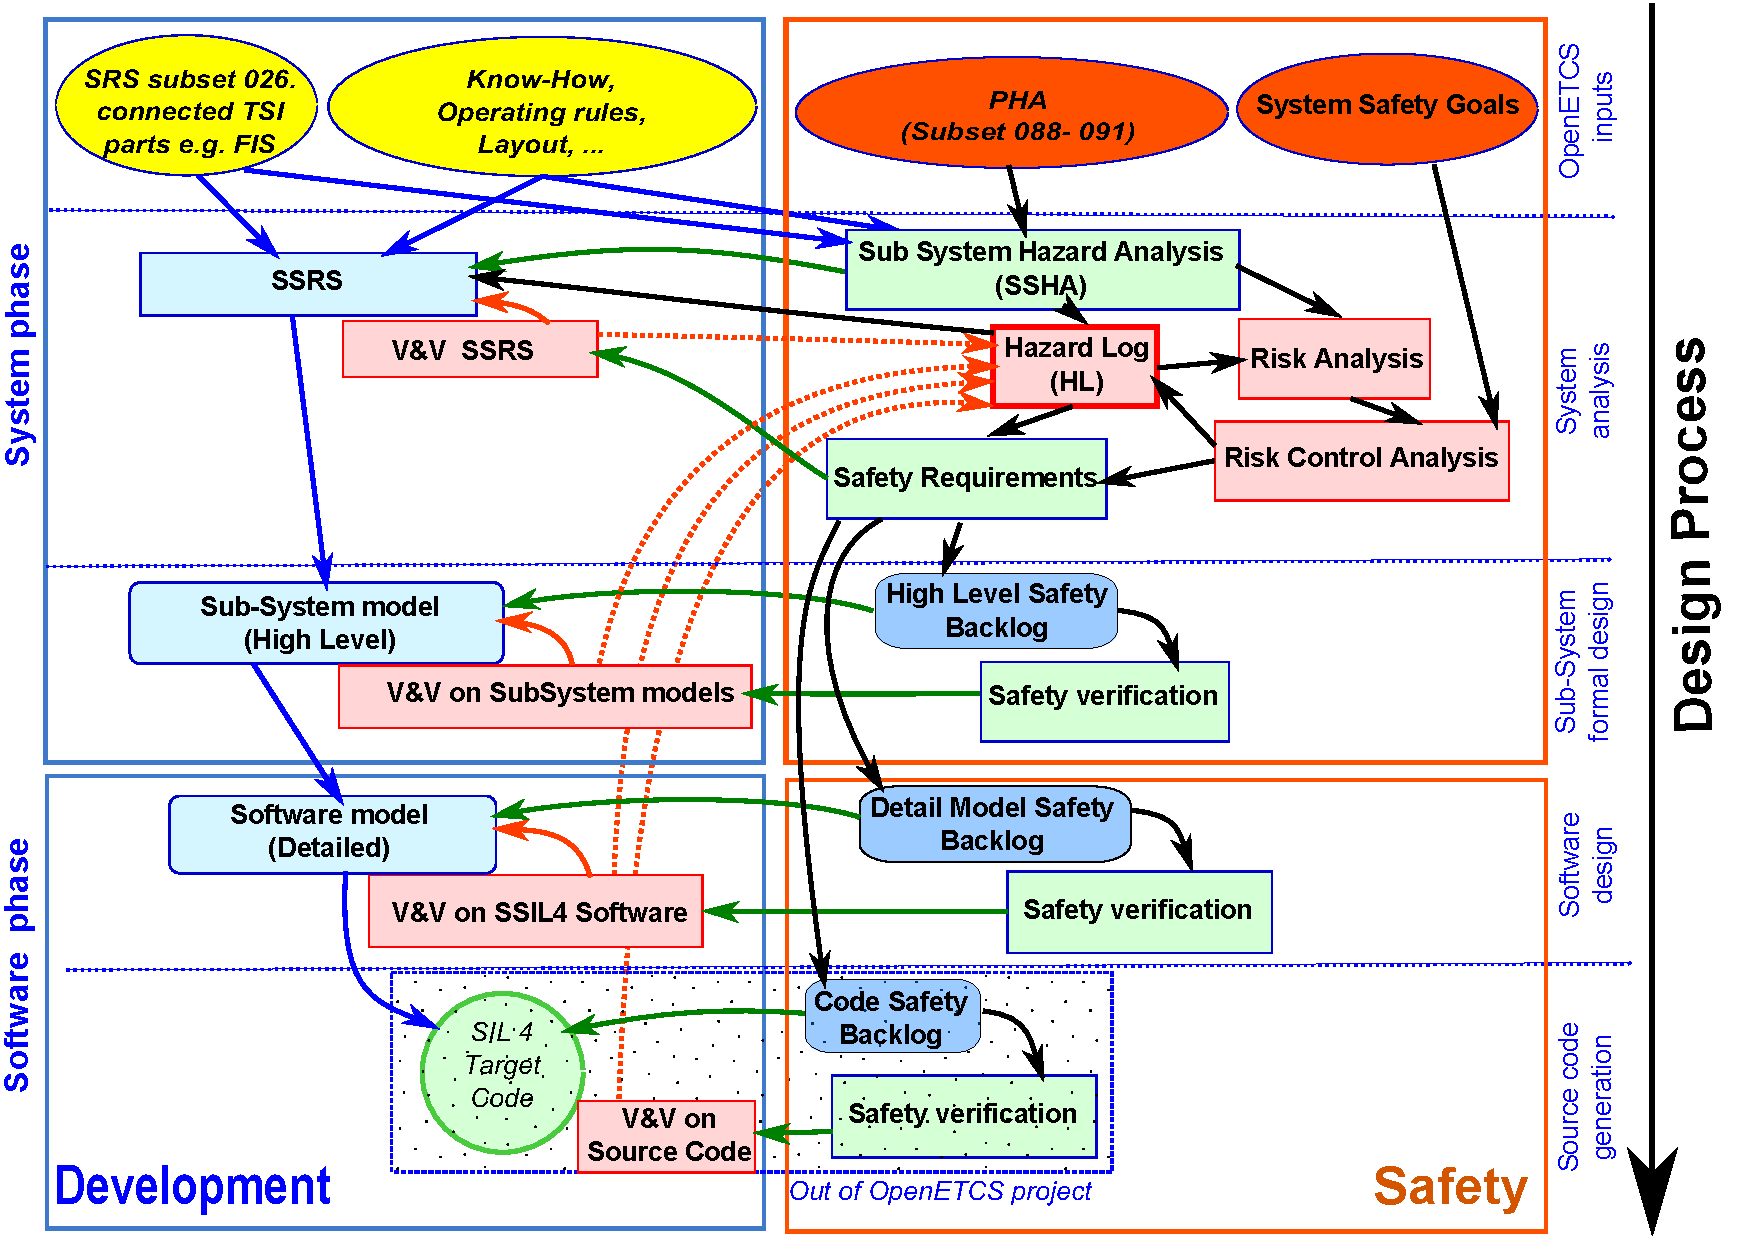
\includegraphics[width=0.7\linewidth]{./figures/WholeSafetyProcess}
\caption[Overall safety process]{Overall safety process}
\label{fig:SafetyProcess}
\end{figure}

\todo[color=yellow!20, inline]{IT: necessary to cover the activities (be sure that are compliant with the Plans), the input and output of each activity and its criteria, entity in charge of each activity and quality activities}

\begin{description}
\item \textbf{System Phase: SSRS}

\underline{\textit{Inputs}}
\begin{itemize}
\item System Requirement Specification SUBSET-026 3.3.0
\item Functional Interface Specification SUBSET-034-3.0.0
\end{itemize}


\underline{\textit{Outputs}}
\begin{itemize}
\item Sub-System Requirement Specification
(SSRS)
\item Application Programming Interface
\item Sub-System Hazard Analyses (SSHA)
\end{itemize}

\underline{\textit{Tasks}}
\begin{itemize}
\item 
\end{itemize}
\end{description}

\begin{description}
\item \textbf{System Phase: Sub-System Model}

\begin{description}
\item semi-formal model of the sub-system
\item strictly formal models
\end{description}

\underline{\textit{Inputs}}
\begin{itemize}
\item 
\end{itemize}

\underline{\textit{Outputs}}
\begin{itemize}
\item sub-system architecture
\item semi-formal model of the sub-system
\end{itemize}

\underline{\textit{Tasks}}
\begin{itemize}
\item Design a model to describe sub-system architecture, main functions and to allocate sub-system requirements
\item completed it with a formal model to focus on a subset of functions or properties
\end{itemize}
\end{description}

\begin{description}
\item \textbf{Software Phase: Software Requirements}

\underline{\textit{Inputs}}
\begin{itemize}
\item 
\end{itemize}

\underline{\textit{Outputs}}
\begin{itemize}
\item 
\end{itemize}

\underline{\textit{Tasks}}
\begin{itemize}
\item 
\end{itemize}
\end{description}

\begin{description}
\item \textbf{Software Phase: Software Model}
\begin{description}
\item semi-formal model 
\item strictly formal model
\end{description}
\underline{\textit{Inputs}}
\begin{itemize}
\item 
\end{itemize}

\underline{\textit{Outputs}}
\begin{itemize}
\item Software Architecture and Design Specification
\item formal model of the software
\end{itemize}

\underline{\textit{Tasks}}
\begin{itemize}
\item 
\end{itemize}
\end{description}

\begin{description}
\item \textbf{Software Phase: Code}

\underline{\textit{Inputs}}
\begin{itemize}
\item 
\end{itemize}

\underline{\textit{Outputs}}
\begin{itemize}
\item 
\end{itemize}

\underline{\textit{Tasks}}
\begin{itemize}
\item 
\end{itemize}
\end{description}

\begin{description}
\item \textbf{Software Phase: V\&V Source Code}

\underline{\textit{Inputs}}
\begin{itemize}
\item 
\end{itemize}

\underline{\textit{Outputs}}
\begin{itemize}
\item SW Code Generation Verification Report
\end{itemize}

\underline{\textit{Tasks}}
\begin{itemize}
\item 
\end{itemize}
\end{description}

\begin{description}
\item \textbf{Software Phase: V\&V Sw model}

\underline{\textit{Inputs}}
\begin{itemize}
\item 
\end{itemize}

\underline{\textit{Outputs}}
\begin{itemize}
\item SW Architecture, Design and Modelling Verification Report
\end{itemize}

\underline{\textit{Tasks}}
\begin{itemize}
\item 
\end{itemize}
\end{description}

\begin{description}
\item \textbf{Software Phase: V \&V Software Requirements}

\underline{\textit{Inputs}}
\begin{itemize}
\item 
\end{itemize}

\underline{\textit{Outputs}}
\begin{itemize}
\item SW Requirements Verification Report
\end{itemize}

\underline{\textit{Tasks}}
\begin{itemize}
\item 
\end{itemize}
\end{description}

\begin{description}
\item \textbf{System Phase: V\&V Subsystem models}

\underline{\textit{Inputs}}
\begin{itemize}
\item 
\end{itemize}

\underline{\textit{Outputs}}
\begin{itemize}
\item 
\end{itemize}

\underline{\textit{Tasks}}
\begin{itemize}
\item 
\end{itemize}
\end{description}

\begin{description}
\item \textbf{System Phase: V\&V SSRS}

\underline{\textit{Inputs}}
\begin{itemize}
\item 
\end{itemize}

\underline{\textit{Outputs}}
\begin{itemize}
\item SSRS verification report
\end{itemize}

\underline{\textit{Tasks}}
\begin{itemize}
\item 
\end{itemize}
\end{description}

\subsubsection{Life Cycle of the OpenETCS Tools chain}
The development of the Tool Chain has to comply with EN50128. Requirements imposed by the standard are analyzed and shown in detail in D2.2. The tools chain development life cycle is described in the document WP7-ToolChainDevelpmentPlan. As the tools chain is a combination and improvement of already existing tools, which have a specific life-cycle, the tools chain life cycle mainly consists of integration and maintenance activities. 

The tool chain lifecycle is depicted figure  \ref{fig:TC_lifecycle}

\begin{figure}[H]
\centering
  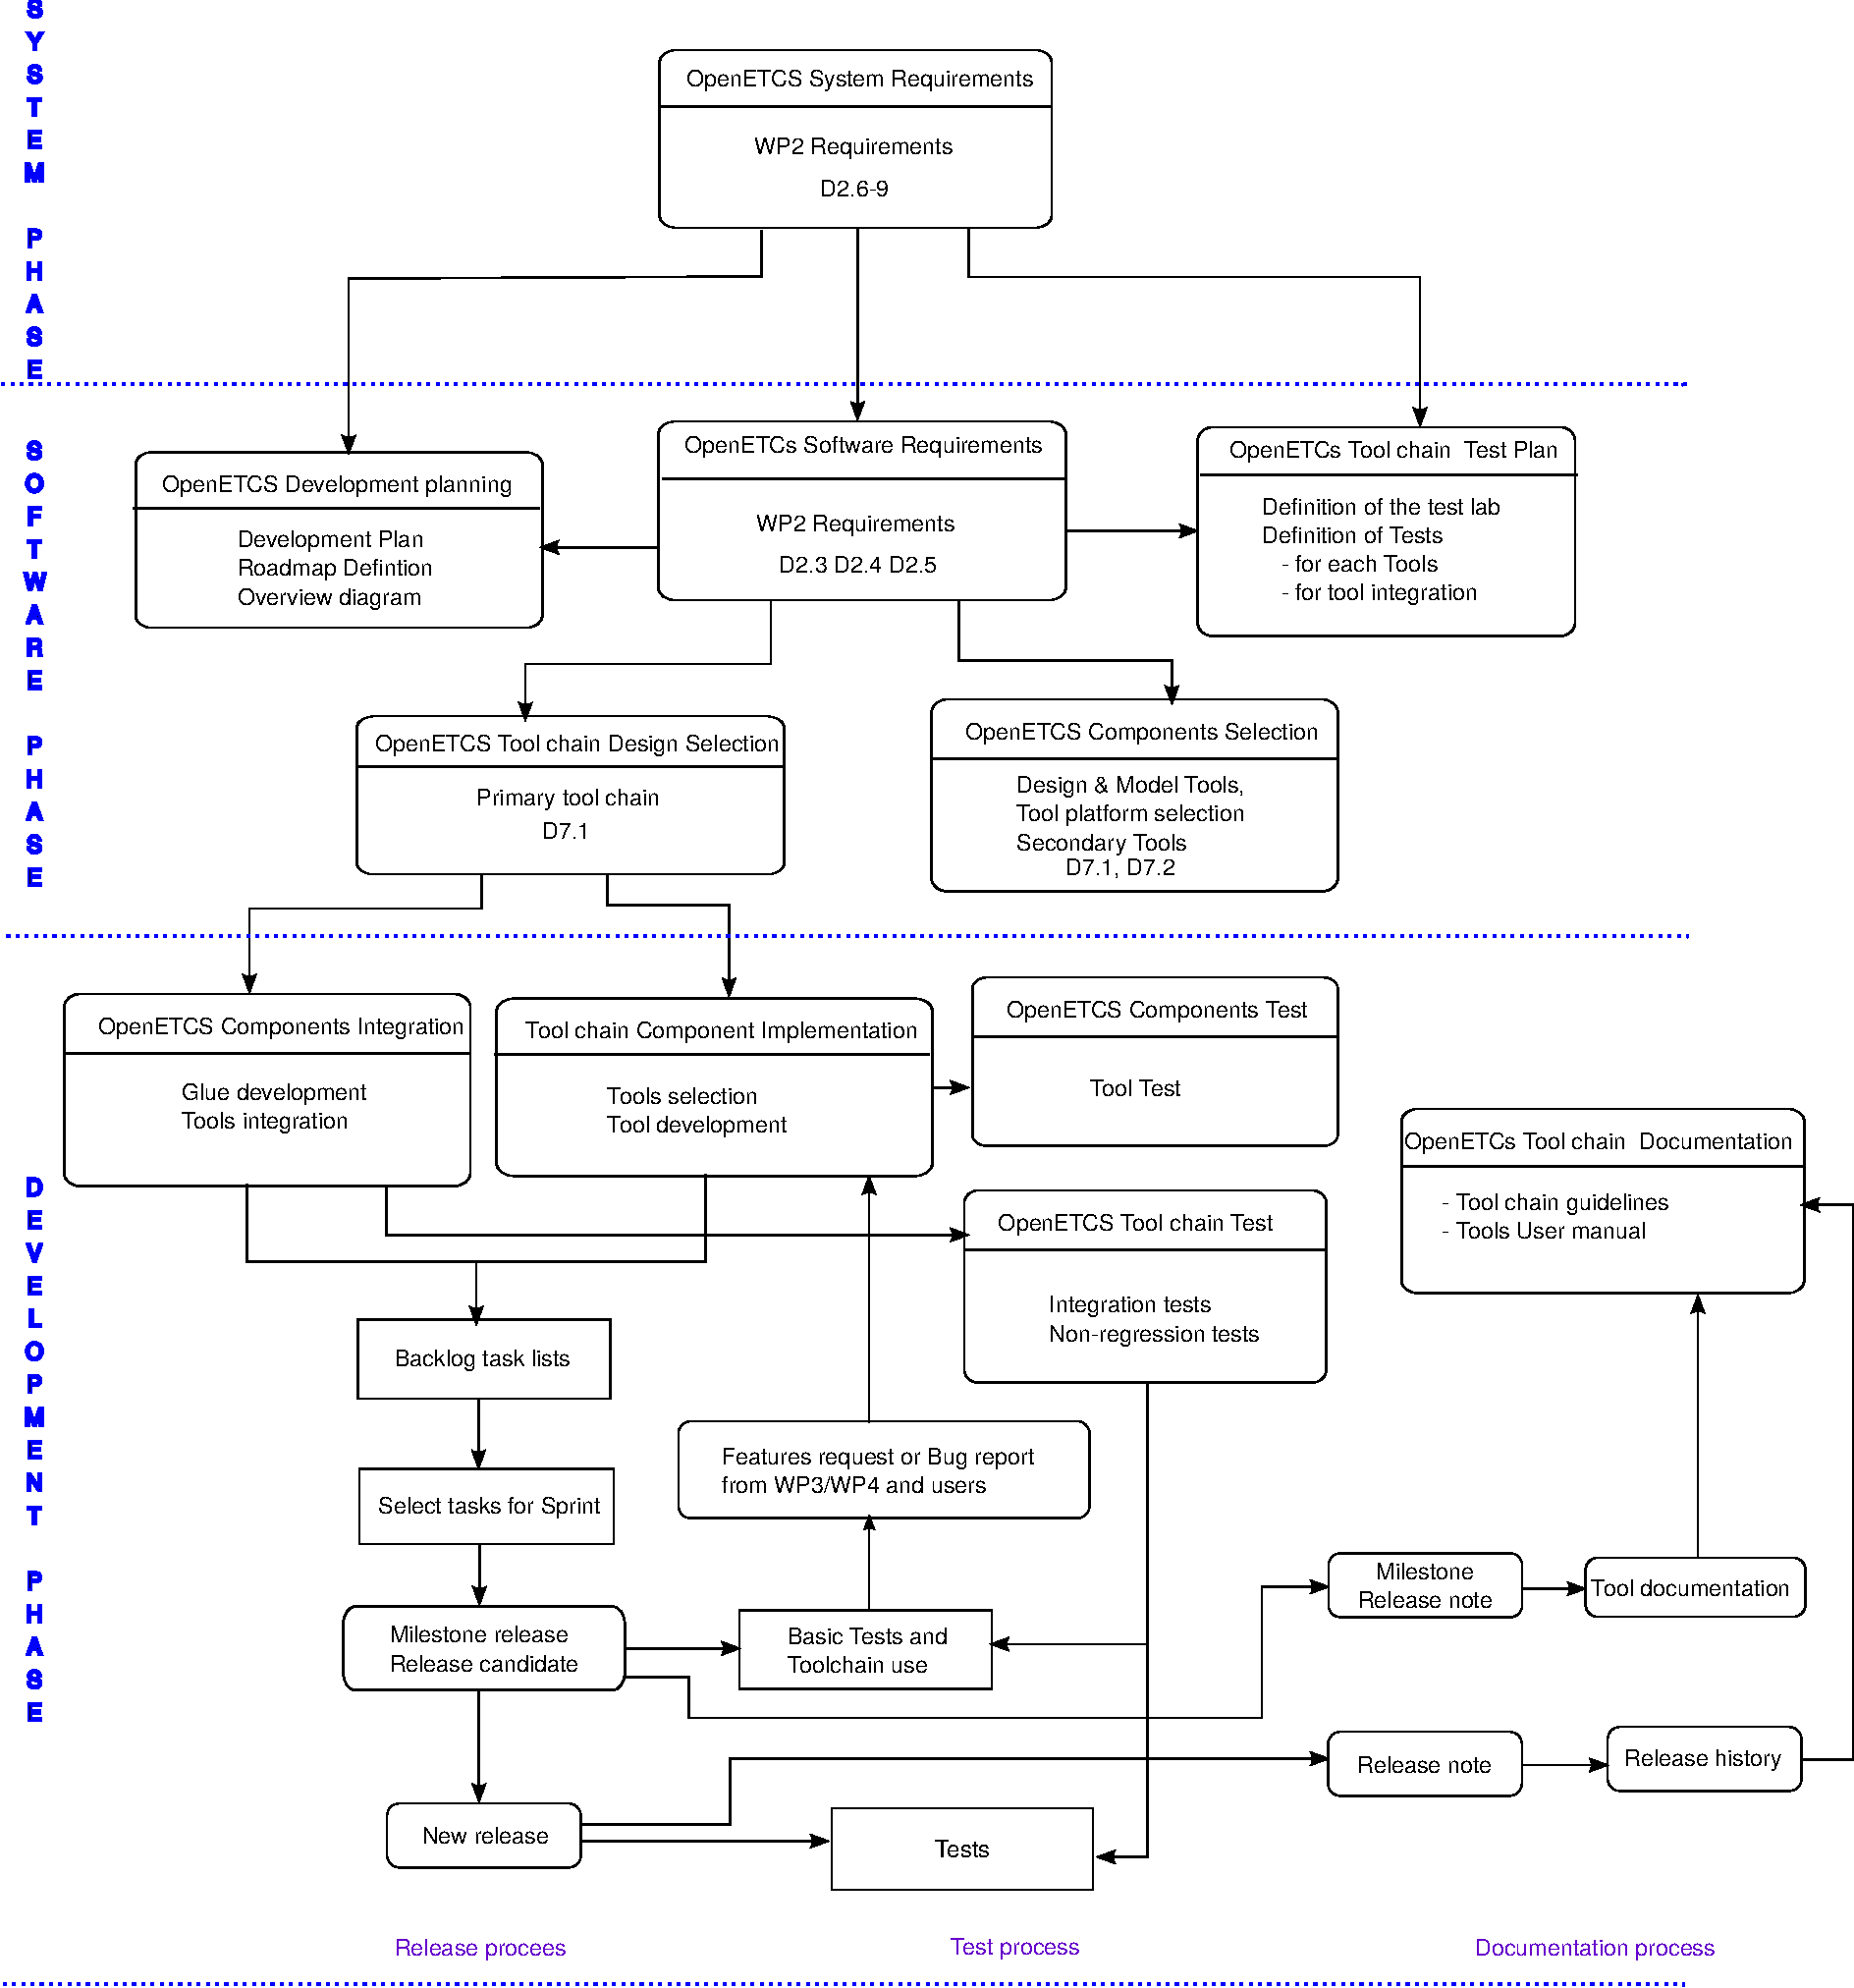
\includegraphics[width= \textwidth]{./figures/toolchain_lifecycle}
  \caption{The OpenETCS tool chain life cycle}
  \label{fig:TC_lifecycle}
\end{figure}

\todo[color=yellow!20, inline]{IT: necessary to cover the activities (be sure that are compliant with the Plans), the input and output of each activity and its criteria, entity in charge of each activity and quality activities}

\textcolor{red}{The following activities will be covered  by the tool chain development.
\begin{itemize}
\item openETCS tool chain architecture specification\\
Definition of the tool chain composition (covers by T7.1 \cite{D7.1}
and T7.2 \cite{D7.2})
\item openETCS tool chain design specification \\
Definition of how the tool chain is implemented including the
definition of the interoperability mechanism
\item Software development\\
Implementation of the tool chain in particular for the need of tool interoperability
\item Test and verification plan\\
Definition of how to test the tool chain.
\item Agile software development guidelines\\
Guidelines on how to use the tool chain in an agile development.
\end{itemize}}

\subsection{QA Management }
The Software quality assurance will assure that any deviations during the project and product life-cycle from plans and standards are detected, recorded, evaluated, tracked, and resolved.

Software quality assurance will work with the Configuration Management process to assure that proper controls are in place and applied to life cycle data.

The monitoring activities of the Life Cycle control involve a development of criteria for inputs and outputs of the different life cycle phases, reviews and documentation audits to determine if the overall Life Cycle process is correctly followed. As well as assuring the compliance with the CENELEC standard.

The QA Manager will be responsible for:
\begin{itemize}
\item Conducting an internal formal audit every month to:
\begin{itemize}
\item assure that the transition criteria to successfully assist in entry from one life-cycle phase to another, is quantifiable, flexible, well documented, and present for every life-cycle phase
\item assure that the different criteria for moving from one step to the next are satisfied (assure transition criteria are adhered to throughout the life-cycle).
\item assure each of the life-cycle phases outputs
are verified, assured, and configured as part of the integral processes (sw verification process, configuration management process, sw quality assurance process, change/problem management process, review and revision processes, ...)
\item Verify the correct aplication of the integral processes inside life cycle
\item ensure that the output deliverables of a phase are consistent and meet all requirements established in the input deliverables
\item assure that the as-delivered products matches the as-built and as-verified product
\item Verify life cycle and assure that every objective and requirement of the CENELEC Standard is fulfilled
\end{itemize}
\item Producing and publishing the corresponding quality reports
\end{itemize}

In order to do the formal review correctly it will be use the Life Cycle Control and Monitoring Activities formal audit checklist. This Checklist template is provided in \href{https://github.com/openETCS/governance/tree/master/Templates}{[governance]}.


\section{Roles}

\newcommand\todoin[2][]{\todo[inline, caption={2do}, #1]{
\begin{minipage}{\textwidth-4pt}#2\end{minipage}}}

\subsection{OpenETCS Roles}

In view of the nature of the project, roles are grouped into three independent categories:

\begin{itemize}
\item CAT1: Open Source Development Process Roles
\item CAT2: SCRUM Roles
\item CAT3: CENELEC Roles 
\end{itemize}

Therefore, any participant will always adopt a role within CAT1, a role within CAT2 and if he/she is involved in the development of a CENELEC assessable product, a third role in CAT3.

As already mentioned, OpenETCS is a project of projects. An expert can participate to different projects with different roles. Therefore an expert will have a CAT1, CAT2 and/or CAT3 role per project.

In the Appendices \ref{ref:CAT1}, \ref{ref:CAT2}, \ref{ref:CAT3S} and \ref{ref:CAT3TC}, the responsibilities and the core competences required by each role are detailed. It is the responsibility of the QA Manager to keep them updated

In the case of CAT 1 roles, specific technical competence will be required depending on the scope of the project. For this reason a new column has been added. In this column, specific technical competences for each project and role are to be included. It is the responsibility of each project leader to provide this information.

According to the open development process followed by Open \gls{ETCS}, the QA process is also a project. For this reason the QA Manager will have to meet the competences of a Project Leader and the specific competences imposed by CENELEC and the OpenETCS project to the Quality Manager activities. When needed, specific responsibilities imposed by a project to a role will be detailed too.

As project results affected by CENELEC are already identified, both core and specific required competence per CAT 3 role are included in Appendices \ref{ref:CAT3S} and \ref{ref:CAT3TC}.

\subsection{Roles within the Development process of the openETCS Software}
The responsibilities and competences for every role specific to the openETCS Software development are listed in Appendix \ref{ref:CAT3S}. The independence of different roles is the core concept of the quality assurance strategy required be CENELEC standard. As openETCS is a collective project by various independent partners, the project organization already ensures full independence between the roles administrated by experts from different partners. 

\subsection{Roles within the Development process of the openETCS Tools Chain}

See Appendix \ref{ref:CAT3TC}
\subsection{QA Activities}

The QA Manager will be in charge of:
\begin{itemize}
\item Maintaining the Requirements Competence Matrices updated in response to the evolution of the OpenETCS project
\item Performing periodical audits of the participants{\textquotesingle} database per project; trace database with the RCM (Required Competence Matrix) for such project
\item Identify training needs and provide the required support to the Project Office in the definition and organization of the corresponding training activities.
\item In the case of CENELEC related project, provide the necessary evidence of competence and independence between roles. If this is not possible, propose the necessary solutions and support the projects in its implementation
\end{itemize}

\section{Methods, measures and tools for quality assurance (product + open \gls{ETCS} software + Tools chain)}


Selection of methods and tools used in each phase of the OpenETCS process is a part of the WP7 activities. This selection is based on the state of art established by WP2 (D2.1 and D2.2), the set of requirements defined by WP2 (D2.6-9) and the process definition (D2.3, D2.4, D4.1, D4.2.3).

Results of the selection of methods and tools are given in the D7.1 and D7.2 deliverables. Conformance of the methods and tools are going to be discussed in D7.3.

The following table give details of all this deliverables.

\begin{table}[H]
\begin{supertabular}{|m{3cm}|m{11cm}|}
\hline
\rowcolor{myblue}
Deliverable &
Content of Relevance for this Chapter\\\hline
D2.1: Report on existing methodologies &
State of the art on methods and tools \\\hline
D2.2: Report on CENELEC Standard &
CENELEC requirements to be fulfilled and the approach followed by the project to provide evidence\\\hline
D2.3: Process definition &
OpenETCS process definition \\\hline
D2.4: Report on Methods definition &
Description of methods and tools to use to follow the OpenETCS process \\\hline
D2.6-9: Set of requirements for the OpenETCS project &
Definition of the requirements that the selected methods and tools shall follow \\\hline
D4.1: Report on \gls{VandV} Plan \& Methodology &
Detailed description of the \gls{VandV} process and how are used the methods and tools to cover \gls{VandV} artifacts \\\hline
D4.2.3: Safety Plan &
Detailed requirements on methods and tools to be used during the process to obtain a \gls{SIL}4 developement of \gls{on-board unit} \\\hline
D7.1: Report on the final choice(s) for the primary tool chain (means of description, tool and platform) &
Selected methods and tools to be used during the specification and design part of the OpenETCS process \\\hline
D7.2: Report on all aspects of secondary tooling (results of T7.2)  &
Selected methods and tools to complete the OpenETCS process (\gls{VandV}, safety analyses,..) \\\hline
D7.3: Tool chain qualification process description &
This report describe how the selected methods and tools fit the qualification requirements according CENELEC standard \\\hline
\end{supertabular}
\caption{Referenced deliverables}
\end{table}


\subsection{Methods, measures and tools for quality assurance OpenETCS Application Software}

It is assumed that the OpenETCS application software will be \gls{SIL}4 compliant. Therefore, the methods, techniques and tools shall be suitable to \gls{SIL} 4. 

The selected methods and measures are included in Appendix  \ref{ref:MethodS}

\subsection{Methods, measures and tools for quality assurance openETCS Tools chain}

The Tool Chain will be composed of a set of tools with different levels of interaction. The openETCS tool chain consists on a series of supporting tools that helps in the development of the whole project. Such tools include, but are not limited to, development and design tools, language translators, testing and debugging tools, and configuration management tools. Support tools are further classified according to their influence on the system:
\begin{itemize}
\item On-line support tools are tools that can directly influence the safety-related system during its run time
\item Off-line support tools are tools that support a phase of the software development lifecycle and that cannot directly influence the safety-related system during its run-time
\end{itemize}

Following CENELEC criteria, each tool belongs to one of the following classes: T1, T2 and T3. Class 3 and Class 2 Tools are obliged to follow specific development methods, techniques and tools. 

%The document D7.3 provides a description of the Tool Chain architecture, jointly with a description of the constituent tools.

\subsubsection{Selected Tools}
\textcolor{red}{See D7.1}

Notes:
\begin{itemize}
\item Eclipse (eclipse Kepler SR1 IDE): tool platform (Eclipse with the modeling framework (EMF))
\item Papyrus/SysML to cover the highest level of the OpenETCS V cycle
\item ProR
\item SCADE
\item EFS to support V\&V activities.
\item Git: configuration management
\end{itemize}


\textcolor{red}{What is the current status of this? SYSML$\backslash$EFS$\backslash$Eclipse Polarsys and SYSML$\backslash$Classical B for final decision on OpenETCS Tools Chain not late than January 2014}

\subsubsection{Metrics Covered by tools}

\begin{table}[H]
\begin{tabular}{|m{3cm}|m{10cm}|}
\hline
\rowcolor{myblue}
\multicolumn{2}{|c|}{T1 Tools} \\\hline
\rowcolor{lightgray}
Name &
Metrics 
\\\hline
ProR & \\\hline
Papyrus & \\\hline
SysML & \\\hline
Git & Software Configuration Management\\\hline
\end{tabular}
\caption{T1 Tools}
\end{table}

\begin{table}[H]
\begin{tabular}{|m{3cm}|m{10cm}|}
\hline
\rowcolor{myblue}
\multicolumn{2}{|c|}{T2 Tools} \\\hline
\rowcolor{lightgray}
Name &
Metrics 
\\\hline
 & \\\hline
\end{tabular}
\caption{T2 Tools}
\end{table}

\begin{table}[H]
\begin{tabular}{|m{3cm}|m{10cm}|}
\hline
\rowcolor{myblue}
\multicolumn{2}{|c|}{T3 Tools} \\\hline
\rowcolor{lightgray}
Name &
Metrics 
\\\hline
 & \\\hline
\end{tabular}
\caption{T3 Tools}
\end{table}


\subsection{Quality Control and Monitoring Activities}
The monitoring activities of the selected Tools, Methods and Techniques implicates a development of criteria, reviews and audits to determine if the overall tools and methods \& Techniques selection and implementation is correctly develop and maintain. As well as assuring the compliance with the CENELEC standard.

The Quality Assurance Manager should do the following monitoring activity:
\begin{itemize}
\item Conduct an internal formal audit to confirm the methods and tools are ready to use. This audit consists in:
\begin{itemize}
\item Assessing the accept criteria of the tools and methods
\item Assessing the fulfilment of the expectations of the tools and methods
\item Assesing the set of selected methods and tools fulfill CENELEC standard (Benchmarking methods, techniques and tools against CENELEC standard.)
\item Verifying every tool availability and operability
\item Verifying new tool version control
\item Verifying the evaluation of the selected tools, methods and techniques
\end{itemize}
\item Conduct an internal formal audit every month to confirm the methods and tools chain are appropiately implemented. 
\begin{itemize}
\item Verifying the correct use of each tool in each WP and Phase
\item Verifying the correct use of each technic and metric in the project
\end{itemize}
\end{itemize}

In order to do the formal review correctly it will be use the Tool, Method and Technic Monitoring Activities formal audit checklist. This Checklist template is provided in \href{https://github.com/openETCS/governance/tree/master/Templates}{[governance]}.

\section{Documentation}

The documentation structure of the OpenETCS project is composed of:
\begin{itemize}
\item Deliverables, which constitute the official outcomes of the different Top-Projects/\gls{WP}s
\begin{itemize}
\item The relation and scope of the deliverables to be produced along OpenETCS can be found in the FPP \citep{fpp}.
\item The updated status of development of each Deliverable can be found in 
\href{https://github.com/openETCS/management/wiki/State-of-Deliverables}{[State-of-Deliverables Wiki]}.
\item The approved and therefore valid version of each Deliverables can be found in the repository of the Top-Project/\gls{WP} it belongs to. 
\end{itemize}
\item Contractual documents, with the Commission and among the project partners
\begin{itemize}
\item The status of development of each contractual document can be found under the repository of Management (WP1).
\item The last approved and therefore valid version of each contractual document can be found under the repository of Management (WP1).
\end{itemize}
\item Periodic Progress Reports, to show progress to ITEA and EC representatives.
\begin{itemize}
\item The state of each Periodic Report can be found under repository of Management (WP1).
\item The last approved and therefore valid version of each Periodic Progress Report can be found under the repository of Management (WP1). 
\end{itemize}
\item Supporting Documents, in the form of Templates and Procedures
\begin{itemize}
\item The procedures and templates applicable to a specific Top-Project/\gls{WP} can be found in the repository of the corresponding TP/\gls{WP}.
\item The procedures and templates applicable to the whole project can be found in the repository of Governance.
\end{itemize}
\item Internal Reports, in the form of Meeting Minutes
\begin{itemize}
\item The minutes of the weekly scrum meetings are found in the repository of Governance.
\end{itemize}
\end{itemize}

The nomenclature used for the naming of the different documents is provided in \href{https://github.com/openETCS/governance/wiki/Nomenclature-Guideline}{[governance Wiki]}.

For each TP/\gls{WP} the relation of existing documents is provided in the form of a list \href{https://github.com/openETCS/governance/wiki}{[Wiki]}. This list includes a direct access to the valid version of each document.

\subsection{Documentation Structure within the development process of the openETCS Software}
As a \gls{SIL}4 software, the documentation structure has to comply with CENELEC requirements. The following table shows the document structure required by CENELEC for a \gls{SIL} 4 development and the corresponding documents produced in the OpenETCS project.

\textcolor{red}{Map the documents with the current openETCS documents and lifecycle}

\begin{center}
\begin{longtable}{|m{2cm}|m{1.5cm}|m{7cm}|m{2cm}|}
\caption{Documentation Structure}\\

\hline \rowcolor{myblue} \multicolumn{4}{|c|}{\textbf{Documentation Structure within the development process of the openETCS Software}} \\ \rowcolor{lightgray} \multicolumn{1}{|c|}{\textbf{Phase}} & \multicolumn{1}{c|}{\textbf{SIL4}} & \multicolumn{1}{c|}{\textbf{Document}} & \multicolumn{1}{c|}{\textbf{Responsible}}\\ \hline 
\endfirsthead

\multicolumn{3}{c}%
{{\bfseries \tablename\ \thetable{} -- continued from previous page}} \\
\rowcolor{myblue} \multicolumn{4}{|c|}{\textbf{Documentation Structure within the development process of the openETCS Software}} \\
\rowcolor{lightgray} \multicolumn{1}{|c|}{\textbf{Phase}} & \multicolumn{1}{c|}{\textbf{SIL4}} & \multicolumn{1}{c|}{\textbf{Document}} & \multicolumn{1}{c|}{\textbf{Responsible}}\\ \hline 
\endhead

\hline \multicolumn{4}{|r|}{{Continued on next page}} \\ \hline
\endfoot

\hline \hline
\endlastfoot

Planning &
\centering \gls{HR} &
Software Quality Assurance Plan

Software Quality Assurance Verification Report

Software Configuration Management Plan

Software Verification and Validation Plan &
\\ \hline
Software Requirements &
\centering \gls{HR} &
Software Requirements Specification

Software Requirements Test Specification

Software Requirements Verification Report &
\\\hline
Architecture and design &
\centering \gls{HR} &
Software Architecture Specification

Software Design Specification

Software Interface Specification
 
Software Integration Test Specification

Software/Hardware Integration Test Specification
 
Software Architecture and design verification report &
\\\hline
Component Design &
\centering \gls{HR} &
Software Component design specification

Software Component Test Specification

Software Component design verification report &
\\\hline
Component Implementation and Testing &
\centering \gls{HR} &
Software source code and supporting documentation

Software source code verification report

Software Component Test Report &
\\\hline
Integration &
\centering \gls{HR} &
Software Integration Test Report

Software/Hardware Integration Test Report

Software Integration Verification Report &
\\\hline
Overall Software Testing/Final validation &
\centering \gls{HR} &
Overall Software Test Report

Software Validation Report

Tools Validation Report
 
Release Note &
\\\hline
Systems configured by Application Data/ algorithms &
\centering \gls{HR} &
Application Requirements Specification

Application Preparation Plan

Application Test Specification
 
Application Architecture and Design
 
Application Preparation Verification Report
 
Application Test Report

Source Code of Application Data/Algorithms
 
Application Data/Algorithms Verification Report &
\\\hline
Software Deployment &
\centering \gls{HR} &
Software Release and Deployment Plan

Software Deployment Manual

Release Notes
 
Deployment Records

Deployment Verification Report &
\\\hline
Software Maintenance &
\centering \gls{HR} &
Software Maintenance Plan

Software Change Records

Software Maintenance Records
 
Software Maintenance Verification Report &
\\\hline
Software Assessment &
\centering \gls{HR} &
Software Assessment Plan
 
Software Assessment Report &
\\\hline
\end{longtable}
\end{center}


\subsection{Documentation Structure within the development process of the openETCS Tools chain}

CENELEC Standard requires that all the off-line support tools have a manual as  minimun required documentation. The Standard also established that tools in classes T2 and T3 should have documentation that defines the behaviour of the tools together with instructions and constrains on its use. This documentation should be a justification for use, a potencial failures identification and the ways to avoid or mitigate them, manuals and use restrictions. It is also required that tools to be assessed with the aim to determine the level of reliance that shall be placed on the tool, and potential failure mechanisms that may affect the executable software (T3 only).

For T3 class applications, evidence shall be available that the tool conforms to its specification or manual, so called tool assessment. Such tool assessment shall cover:
\begin{itemize}
\item A chronological record of the validation activities
\item The version of the tool product manual being used
\item The tool functions being validated
\item Tools and equipment used
\item The results of the validation activity; the documented results of validation shall state either that the software has passed the validation or the reasons for its failure
\item Test cases and their results for subsequent analysis
\item Discrepancies between expected and actual results
\end{itemize}

It is important to add, that every new version of a support tool shall be certified. This may rely on evidence provided for earlier versions if sufficient evidence provides that the modifications do not affect tool compatibility with the rest of the tools in the integrated tool chain and that the new version is unlikely to contain significant new, unknown faults.

\textcolor{red}{create a similar table than in section 6.1 for the tool chain documentation}

\subsection{Quality Control and Monitoring Activities}
The monitoring activities of the Documentation Structure control involves a development of  criteria, reviews and documentation audits to determine if the overall structure of the documentation is correctly followed. As well as assuring the compliance with CENELEC standard for a SIL 4 product.

The Quality Assurance Manager should do the following monitoring activity:
\begin{itemize}
\item Conduct an internal formal audit every month to confirm the documentation structure is maintained correctly. This audit consists in:
\begin{itemize}
\item Verifying each document development in time and its correct classification inside the WP and Phase.
\item Controlling the document version labels and identifier
\item Benchmarking against CENELEC standard (verifying life cycle and assuring that every objective and requirement of the CENELEC Standard is fulfilled)
\item Assessing the document timeline’s creation
\end{itemize}
\item Produce and publish the corresponding quality reports
\end{itemize}

In order to do the formal review correctly it will be use the Document  Structure Control and Monitoring Activities formal audit checklist. This Document Structure Checklist template is provided in \href{https://github.com/openETCS/governance/tree/master/Templates}{[governance]}.

\section{Documentation Control}
The Documentation Control procedure describes the steps to follow to ensure that the documentation developed whiting the openETCS project is current and suitable for use by the Eclipse community, the project members and the key customers. The main control activities covered by the procedure include the document creation and review, the approval, dissemination, archiving, modification and update due to a change request or the monitoring of the evolution among the time among others.

The implementation of this procedure, shall ensure that openETCS documents can be located easily, be periodically reviewed, have the nomenclature updated when needed, be available at any time, and be moved and archived when they are labelled ad obsolete.

The whole procedure is fully described in the \href{https://github.com/openETCS/governance/tree/master/Document%20Control%20Process}{[Document Control Procedure]} .

There is a signature copy inside the project office mandatory for all official deliverables and selected additional documents. The selection of the documents to be signed signed is in the resposibility of the workpackage leader

\subsection{Quality Control and Monitoring Activities}
The monitoring activities of the Documentation Control, carried on by the Quality Assurance Manager, implicate an in-depth analysis of the document development process. This analysis involves developing criteria, conducting reviews and examining documentation to determine how the process is conducted.

The Quality Assurance Manager should do the following monitoring activity:
\begin{itemize}
\item Conduct an internal formal review every 2 months to confirm the documentation control is done correctly. This review consists in:
\begin{itemize}
\item Verifying each document correct location and labeling in the GITHUB repository
\item Verifying the roles of the documentation.
\item Verifying that the terminology, acronyms or abbreviations have the same meaning in every document
\item Verifying the document schedule fulfillment
\item Controlling obsolete documentation labels and location
\item Benchmarking compliance with CENELEC standard
\item Assessing that every document applies the conditions and requirements of the preceding document with which it has a hierarchical relationship. It should not be contradictions among the documentation and its preceding documents
\item Assessing that there is a reference with the same name and description for each element or concept in every document
\end{itemize}
\item Conduct an internal informal review every month using the plans, goals and objectives established in the project to verify control documentation and documentation development is done satisfactorily.
\item Participate in the review processes of the different documents
\item Maintain a set of metrics for the Document Control process.
\item Produce and publish the corresponding quality reports.
\end{itemize}

In order to do the formal review correctly it will be use the Document Control and Monitoring Activities formal review checklist.  This Document Control Checklist template is provided in \href{https://github.com/openETCS/governance/tree/master/Templates}{[governance]}.

\section{Tracking and tracing of deviation}

\subsection{Traceability (openETCS software + Tools chain)}

The monitoring activities of the Traceability help to determine how the traceability among the different elements of the project is conducted. In order to have a good traceability, it has been established to develop a traceability matrix. 

During the whole project different traceability matrix will be used and all of them will monitor in the same way.

The Quality Assurance Manager should do the following monitoring activity:
\begin{itemize}
\item Verify that the means to demonstrate traceability throughout all phases of the lifecycle are provided
\item Verify that the output of the traceability process is the subject of formal configuration management
\item Verify that the requirements traceability is covered completely
\item Assure that any untraceable material (requirement, model, code, ...) to have no bearing upon the safety or integrity of the system
\item Ensure that each specific CENELEC role is responsible for establishing and maintaining traceability to and from the specific elements.
\item Monitor the different matrix with informal reviews every month and with formal reviews every 3 months. These reviews will consist in assuring that the generated matrix table has well traced every element of the project.

In order to do this the following relations among elements will be reviewed:
\begin{enumerate}
\item Traceability between requirements and models (design)
\item Traceability between models and the generated code
\item Traceability among requirements, models, test plans, specifications to the test or other reports which record the results of their application and tool chain.
\end{enumerate}
\end{itemize}

In order to do the formal review correctly it will be use the Traceability Activities formal review checklist. This Traceability Checklist template is provided in \href{https://github.com/openETCS/governance/tree/master/Templates}{[governance]}.

\subsection{Configuration Management}

Configuration Management (CM) is used to handle changes systematically so that a system maintains its integrity over time. The Software Configuration Management Plan  \href{https://github.com/openETCS/governance/blob/master/SCMP/SCMP_0.0.0.pdf}{[SCMP]} \cite{scmp} defines the procedures, techniques, and tools that are required to manage the software development, evaluate proposed changes, trace the status of changes, and to support an inventory of the system. 

The main points to perform the configuration management process are:

\vspace{-10pt}
\begin{itemize}
\item Configuration Management Tools
\item Configuration Items
\item Configuration Management Organization
\item Configuration Control/Change Management
\item Configuration Audits
\item Baselines
\end{itemize}

The Quality Assurance Manager is accountable for the implementation of the \gls{SCMP}.

The QA Manager will be in charge of:
\begin{itemize}
\item perform periodical audits
\begin{itemize}
\item Audits to verify the process itself: the correct implementation of the process and the compliance of the process with CENELEC Standard
\end{itemize}
\item Produce and publish the corresponding quality reports.
\end{itemize}

\subsection{Fault Management}

A failure is a deviation of the component or system from its expected delivery, service or result. A failure is the consequence of a fault or error in a system but not all faults result in failures.

Faults, failures and errors encountered during the review activities (QA. Verification, Validation, Assessment) planned in the software development life-cycle, problems reported by users and customers as well as change requests initiated by any of the system stakeholders will be reported and managed following the Change/Problem Management Process  \citep{emp} detailed in \href{https://github.com/openETCS/governance/tree/master/Change-Problem%20Process}{[governance]} and through the Change/Problem Management Tool. This tool will be integrated with the Configuration management tool {\it GIT} and will be configured to implement and record all the information generated during the process.

The integration with the Configuration management tool {\it GIT} will permit:
\begin{itemize}
\item Traceability between Change/Problem Requests and the configuration items where the problem was located.
\item Traceability between the configuration items modified and the corresponding Change/problem request. 
\end{itemize}
 
The implementation of the workflow will permit:
\begin{itemize}
\item A complete history trail of the Change Request/Problem Report
\end{itemize}

The purpose of the Change/Problems Management implementation at OpenETCS project is to ensure that standardized methods and procedures are used for efficient and prompt handling of all changes/problems associated with the OpenETCS products, in order to minimize the number and impact of any related changes/problems. Changes/problems in the products may arise reactively in response to incidents, or proactively from seeking improved efficiency and effectiveness, as well as to enable or reflect OpenETCS initiatives, or products improvements.

The QA Manager will be in charge of:
\begin{itemize}
\item perform periodical audits and quality assessments of the bugs received
\begin{itemize}
\item Audits to verify the process itself
\item Quality Assessments to verify the evolution of the product quality
\end{itemize}
\item Assist in determining QA impacts
\item Support Problem owner in analysis
\end{itemize}

\subsection{Grievance Handling}

It is a good culture to solve concerns as close as possible to the root cause of an problem or a misunderstanding. This means, the team where a problem is seen first is empowered to search for a solution of the problem first.

If the partners cannot agreed on a solution, the impediment is escalated to the next level in the project hierarchy. 

When a member of the openETCS community has a concern about a Project, the  member will raise that concern with the Project's Leadership (e.g., task leader in openETCS). If the member is not satisfied with the result, the member can raise the concern with the parent Project's Leadership, typically the workpackage leader.

The Member can continue appeals up the Project Leadership Chain and, if still not satisfied, thence to the project management board PMB, then the openETCS project lead, and finally to the project co-operation committee (PCC). All appeals and discussions will abide by the Guiding Principles of being open, transparent, and public.

Member concerns may include:
\begin {itemize}
\item Out of Scope. It is alleged that a Project is exceeding its approved scope.

\item Dysfunctional. It is alleged that a Project is not functioning correctly or is in violation of one or more requirements of the Development Process.\

\item Contributor Appeal. It is alleged that a Contributor who desires to be a Committer is not being treated fairly.

\item Invalid Veto. It is alleged that a -1 vote on a Review is not in the interests of the Project and/or of Eclipse.
\end{itemize}

A variety of grievance resolutions are available to the PMB up to, and including, rebooting or restarting a project with new Committers and leadership.

The issues seen during a sprint shall be taken to the sprint retrospective in order to help the team find an easy way in the future.

\subsection{Software Maintenance}
\subsubsection{Software Maintenance Plan}
Software Maintenance Plan introduces the approach that the OpenETCS-Software and OpenETCS-Toolchain project adopts for the maintenance of the software components.

The procedures for software maintenance will be contained in the Software Maintenance Plan for OpenETCS-Software (SMP-SW) and the Software Maintenance Plan for OpenETCS-ToolChain (SMP-toolchain). These procedures should also contain information about:
\begin{itemize}
\item Control of the error report, the error log, maintenance records, authorizations to make changes and software configuration / system and the techniques for estimation impact analysis and record and data analysis.
\item Evaluation, Verification and Validation of every change
\item Definition of software modification process (definition of the Authority which approves the changed software, etc...)
\end{itemize}


\subsubsection{Modification and change control }

A change is the addition, modification, or removal of a configuration item (CI), product, or product component, and/or its associated elements

The change requests initiated by any of the system stakeholders will be reported and managed following the Change/Problem Management Process  \citep{emp} detailed in \href{https://github.com/openETCS/governance/tree/master/Change-Problem%20Process}{[governance]} and through the Change/Problem Management Tool.

The Change/problem Management process aims to evaluate and plan the change/problem process to ensure that, if a change is made, it is done in the most efficient way possible, following the established procedures and ensuring the quality and continuity of the OpenETCS project and products at all times.

The Change/problem Management process should define at least the following:
\begin{itemize}
\item the necessary documentation to report a problem
\item analysis of the collected information
\item practices to be followed to report, track and resolve identified problems
\item responsabilities 
\item controls to ensure that corrective actions have been taken and are effective
\item impact analysis
\item approval before implementation
\end{itemize}

\subsubsection{Quality control and monitoring activities}
For Software Maintenance the following metrics to follow in order to control the Maintenance phase are identified:
\begin{itemize}
\item Maintenance efficiency
\item Maintenance effectiveness
\end{itemize}

Any trends and changes that occur provide an analytical basis for managerial decision making, regarding issues such as; examining resource requirements and initiation of corrective and preventive actions. 

The QA Manager will be in charge of:
\begin{itemize}
\item perform periodical audits and quality assessments of the change request received
\begin{itemize}
\item Audits to verify the processes themself: the correct implementation of the processes and the compliance of the processes with CENELEC Standard
\item Quality Assessments to verify the evolution of the product quality
\end{itemize}
\item Assist in determining QA impacts
\item Support Change owner in analysis
\end{itemize}


\section{Supplier Control}


This section describes what openETCS consortium expects its suppliers to do to
ensure that all openETCS products' requirements and expectations are met.

This Supplier control applies to all Suppliers providing openETCS project with materials, products, processing, and related services.

At following, the expected Suppliers' general requirements are listed:

\begin{itemize}
\item Supplier shall ensure the confidentiality of openETCS project and products under development, and related product information, as well as \gls{intellectual property} shared as a result of the working relationship.
\item Suppliers are expected to have an effective quality system that ensures conforming product is delivered.
\begin{itemize}
\item Suppliers shall maintain a Quality Management System suitable to the products and services provided to openETCS, that is certified by an accredited third-party certification body, i.e. ISO9001. This letter of accreditation should be provided to the respective QA personnel
\item In the absence of third-party certification, depending on the product, its application, value, and criticality, the OpenETCS community and Quality Assurance Manager may authorize the acceptance of other evidence of compliance
\end{itemize}
\item Supplier should assure that all performance, endurance, maintenance, safety and warning requirements are met.
\item The Supplier shall maintain documented procedures for identification of product from receipt and during processes of production and delivery. When traceability is a specified requirement, the Supplier shall establish and maintain a documented procedure for unique identification of individual product or batches
\item The supplier shall provide and maintain suitable gauges, measuring instruments and test equipment to measure/test all material for conformance to OpenETCS requirements.
\item Copies of quality conformance inspection data pertinent to material inspection must be provided by the supplier if required for each shipment or retained at Suppliers premises for future verification.
\item The Supplier shall provide evidence that the following verifications required by the design record and control plan have been completed and that results indicate compliance with specified requirements
\item Suppliers will be responsible for corrective action when changes to product specifications without prior notification to QA result in non- conformity to product or processes.
\item OpenETCS requires all Suppliers to be approved prior to the issuance of contracts
\end{itemize}

\paragraph{Supplier Approval Process}
\begin{itemize}
\item \textbf{Registration:} New suppliers must complete a registration form. This form initiates the approval 
\item \textbf{Evaluation:} 
\begin{itemize}
\item Ensure Supplier Risk Assessment considers both:
\begin{itemize}
\item \underline{Quality risk}
\begin{itemize}
\item Finished Device Quality implications
\end{itemize}
\item \underline{Supply risk}
\begin{itemize}
\item Including implications of supplier going out of business
\end{itemize}
\end{itemize}
\item Evaluate Suppliers using Questionnaires, Self surveys and Audits techniques
\item Supplier’s grading based upon evaluation results and assigned an evaluation status: Approved, conditional or not approved
\end{itemize}
\item \textbf{Certification}: Classify Suppliers based on both QUALITY Risk and SUPPLY Risk.
\end{itemize}

The QA Manager will be in charge of:
\begin{itemize}
\item inspect records/evidence of a supplier’s quality management systems at their facility
\item monitoring and feedback processes: Include periodic review of critical product/process data
\item documents problem issues and requirements for the supplier
\item analyses the supplier operating conditions,
\item Establish Minimal performance for Quality and Delivery
\item When a supplier provides a product/part, apply supplemental controls to further mitigate risk 
\begin{itemize}
\item Product Acceptance Activities
\item Supplier Performance and Monitoring: augmented frequency of reviews
\end{itemize}
\item creates a corrective development profile together with the supplier,
\end{itemize}


\section{Publishing Guideline}
\label{sct:publishingguideline}

\begin{figure}[H]
\includegraphics[trim=1.5cm 7cm 2cm 0,clip,width=\textwidth]{figures/publication_process_bpmn}
\caption{The publishing process as BPMN diagram}
\label{fig:process}
\end{figure}

When publishing in the context of the openETCS project authors shall adhere to this guideline. Figure~\ref{fig:process} depicts the steps as graphical BPMN process. The individual steps are described in detail in the following.

\begin{enumerate}
  \item  It must be ensured that the \emph{project}, the \emph{funding authority} and the \emph{grant number} is mentioned in the paper/presentation. The following acknowledgements can be used:
  \begin{description}
    \item[Germany] This work was funded by the German Federal Ministry of Education and Research (Grant No. 01IS12021) in the context of the ITEA2 project openETCS.
    \item[Belgium/Brussels region] This work was funded by the Région de Bruxelles-Capitale / Brussels Hoofdstedelijk Gewest (Grant No. RBC/12 R 11) in the context of the ITEA2 project openETCS.
    \item[Belgium/Walloon region] This work was funded by the Walloon Region (DG06) (Grant No. 6921) in the context of the ITEA2 project openETCS.
    \item[France] This work was funded by the "Direction Générale de la compétitivité, de l’industrie et des services" (DGCIS)  (Grant No. 112930309) in the context of the ITEA2 project openETCS.
    \item[Spain] This work was funded by the "Gobierno de España, Ministerio de Ciencia e Innovación" in the context of the ITEA2 project openETCS
  \end{description}

\item Publications potentially affecting project contributions of other partners require explicit approval. A request for approval shall be accompanied with a reasonable deadline (e.g., two weeks). Please consider a joint publication with the involved partners.

\item An entry with the details of the publication should be added to the Zotero group \emph{openETCS Publications} by using the Zotero tool or the website \href{http://www.zotero.org}{zotero.org}. A how-to regarding the use of Zotero in openETCS is \href{https://github.com/openETCS/Dissemination/wiki/Management-of-Publications-and-References-with-Zotero}{provided here}. A link to an official and public webpage where the publication can be obtained/purchased should be included.

\item The final document should be uploaded to GitHub to one of the following directories:
  \begin{itemize}
    \item To \href{https://github.com/openETCS/dissemination-management/tree/master/ProjectPublications}{Dissemination-Management/ProjectPublications} if legal restrictions apply for publication.
    \item To \href{https://github.com/openETCS/Dissemination/tree/master/ProjectPublications}{Dissemination/ProjectPublications} if it can be published freely under the openETCS Open License.
  \end{itemize}
\end{enumerate}

\section{Perimeter of the System}
\subsection{List of Functions}
%See \href{https://github.com/openETCS/SRS-Analysis/blob/master/System%20Analysis/List_Functions.xlsx}{List of functions} to complete it

\begin{center}
\begin{longtable}{|m{1.5cm}|m{9cm}|m{3cm}|m{2cm}|}
\caption{Functions}\\

\hline \rowcolor{myblue} \multicolumn{4}{|c|}{Functions} \\ \rowcolor{lightgray} \multicolumn{1}{|c|}{Number} & \multicolumn{1}{|c|}{Name} & \multicolumn{1}{|c|}{Block/ Function} & \multicolumn{1}{|c|}{Complexity}\\ \hline 
\endfirsthead

\multicolumn{4}{c}%
{{\bfseries \tablename\ \thetable{} -- continued from previous page}} \\
\hline \rowcolor{myblue} \multicolumn{4}{|c|}{Functions} \\ \rowcolor{lightgray} \multicolumn{1}{|c|}{Number} & \multicolumn{1}{|c|}{Name} & \multicolumn{1}{|c|}{Block/ Function} & \multicolumn{1}{|c|}{Complexity} \\ \hline
\endhead

\hline \multicolumn{4}{|r|}{{Continued on next page}} \\ \hline
\endfoot

\hline \hline
\endlastfoot

\rowcolor{orange}
1 & DataPreparation & B & \\\hline
1.1 & Board\_External\_Interface & F & \\\hline
\rowcolor{orange}
1.2 & GATC TRAINBORNE SUB SYSTEM & B & \\\hline
1.2.1 & Filter\_information\_from\_ERTMS\_trackside (including linking) & F & 3 \\\hline
\rowcolor{orange}
1.3 & Provide\_automatic\_train\_protection & B & \\\hline
1.3.1 & Manage\_STMs & F & 3 \\\hline
1.3.2 & Determine\_train\_location\_information & F & 3 \\\hline
1.3.3 & Control\_route\_suitability  & F & 1 \\\hline
1.3.4 & Manage\_track\_conditions & F & 2 \\\hline
\rowcolor{orange}
2 & Ensure\_train\_protection & B & \\\hline
2.1 & Manage\_reception\_of\_MA\_information  & F & 2\\\hline
2.2 & Manage\_TSR & F& 1\\\hline
2.3 & Manage\_Speed\_Supervision\_Inputs & F & 2 \\\hline
\rowcolor{orange}
2.4 & Active\_and\_Manage\_train\_protection & B & \\\hline
2.4.1 & Activate\_train\_protection\_in\_FS & F & 3\\\hline
2.4.2 & Activate\_train\_protection\_in\_OS & F & 3\\\hline
2.4.3 & Activate\_train\_protection\_in\_LS & F & 3\\\hline
2.4.4 & Activate\_train\_protection\_in\_SR & F & 2\\\hline
2.4.5 & Activate\_train\_protection\_in\_UN & F & 2\\\hline
2.4.6 & Activate\_train\_protection\_in\_SH & F & 2\\\hline
2.4.7 & Activate\_train\_protection\_in\_TR & F & 2\\\hline
2.4.8 & Activate\_train\_protection\_in\_SF & F & 1\\\hline
2.4.9 & Activate\_train\_protection\_in\_SB & F & 2\\\hline
2.4.10 & Activate\_train\_protection\_in\_PT & F & 2\\\hline
2.4.11 & Activate\_train\_protection\_in\_RV & F & 2\\\hline
2.4.12 & Activate\_train\_protection\_in\_IS & F & 1\\\hline
2.4.13 & Perform train protection & F & 3\\\hline
2.4.14 & Perform train protection related actions & F & 3\\\hline
2.4.15 & Activate\_train\_protection\_in\_SN & F & 2\\\hline
2.4.16 & Activate\_train\_protection\_in\_PS & F & 2\\\hline
2.4.17 & Activate\_train\_protection\_in\_NP & F & 1\\\hline
2.5 & Manage\_emergency\_stop\_messages & F & 2\\\hline
\rowcolor{orange}
3 & Manage\_mode\_and\_level\_and\_procedures\_and\_ancillary\_functions & B & \\\hline
3.1 & compute\_mode & F & 2\\\hline
3.2 & compute\_level & F & 2\\\hline
\rowcolor{orange}
3.3 & Manage\_procedures & B & \\\hline
3.3.1 & capture\_data\_for\_mission & F & 2\\\hline
3.3.2 & handle\_mode\_profile\_procedure & F & \\\hline
3.3.3 & handle\_SH\_procedure & F & \\\hline
3.3.4 & handle\_RV\_procedure & F & \\\hline
3.3.5 & handle\_override\_EOA & F & \\\hline
\rowcolor{orange}
3.4 & Perform\_ancillary\_functions & B & \\\hline
3.4.1 & Manage\_track\_ahead\_free & F & 2\\\hline
3.4.2 & Display\_text\_messages\_coming\_from\_trackside & F & 1\\\hline
3.4.3 & Display\_geographical\_position & F & 1\\\hline
3.4.4 & End\_mission & F & 1\\\hline
3.4.5 & Manage\_national\_values & F & 1\\\hline
3.4.6 & store\_configuration\_data & F & 1\\\hline
3.4.7 & Management of MA request & F & 2\\\hline
3.4.8 & Sending of position report & F & 1\\\hline
3.4.9 & Determine train integrity & F & 1\\\hline
3.4.10 & Detect\_change\_of\_orientation & F & 2\\\hline
3.4.11 & Manage\_cold\_movement\_detection & F & 1\\\hline
3.4.12 & Provide\_train\_movement information & F & \\\hline
3.4.13 & Manage\_radio\_sessions & F & \\\hline
3.4.14 & Record\_juridical\_data & F & 2\\\hline
3.4.15 & Interface with train & F & 2\\\hline
3.4.16 & Interface with DMI & F & 2\\\hline
\end{longtable}
\end{center}


\subsection{List of Risks}

\begin{center}
\begin{longtable}{|m{3cm}|m{13cm}|}
\caption{Risks}\\

\hline \rowcolor{myblue} \multicolumn{2}{|c|}{Risks} \\ \rowcolor{lightgray} \multicolumn{1}{|c|}{Event Id.} & \multicolumn{1}{|c|}{Event Description} \\ \hline 
\endfirsthead

\multicolumn{2}{c}%
{{\bfseries \tablename\ \thetable{} -- continued from previous page}} \\
\hline \rowcolor{myblue} \multicolumn{2}{|c|}{Risks} \\ \rowcolor{lightgray} \multicolumn{1}{|c|}{Event Id.} & \multicolumn{1}{|c|}{Event Description} \\ \hline
\endhead

\hline \multicolumn{2}{|r|}{{Continued on next page}} \\ \hline
\endfoot

\hline \hline
\endlastfoot

MMI-1a & False acknowledgement of mode change to less restrictive mode \\\hline
MMI-1b & False command to enter Non-leading mode \\\hline
MMI-1c & False command of Override request \\\hline
MMI-1d & False acknowledgement of Level Transition \\\hline
MMI-1e & False acknowledgement of Train Trip \\\hline
MMI-1f & False acknowledgement of Track Ahead Free \\\hline
MMI-1g & False shunting request \\\hline
MMI-1h & False acknowledgement of undesired train movement (RAP, RMP and SSS) \\\hline
MMI-2a.1 & False presentation of train speed on the DMI \\\hline
MMI-2a.2 & False presentation of speed (except train speed) or distance on the DMI, including supervision status \\\hline
MMI-2b & False presentation of mode on the DMI \\\hline
MMI-2c & False presentation of track adhesion \\\hline
MMI-2d & Failure to present Entry in FS/OS informa-tion \\\hline
MMI-2e & False presentation of train data/additional data \\\hline
MMI-2f & False presentation of Override status, including false enabling of override selection \\\hline
MMI-2g & Failure to present acknowledgement message to a less restrictive mode \\\hline
MMI-2h & False presentation of TAF request \\\hline
MMI-2i & Failure to present LX “not protected” infor-mation \\\hline
MMI-2j & False presentation of reversing allowed \\\hline
MMI-2k & False presentation of level transition an-nouncement\\\hline
MMI-3 & Falsification of driver's train data / addi-tional data input stored onboard \\\hline
MMI-4 & Falsification of SR speed/distance data \\\hline
MMI-5 & Falsification of train integrity input \\\hline
MMI-6 & Falsification of Virtual Balise Cover \\\hline
ODO-1 & Incorrect standstill indication \\\hline
ODO-2 & Speed measurement underestimates trains actual speed \\\hline
ODO-3 & Incorrect actual physical speed direction \\\hline  
ODO-4 & The confidence interval for distance measurement does not include the real position of the train \\\hline
KERNEL-1 & Balise linking consistency checking failure \\\hline
KERNEL-2 & Balise group message consistency checking failure \\\hline
KERNEL-3 & Failure of radio message correctness check \\\hline
KERNEL-4 & Radio sequencing checking failure \\\hline
KERNEL-5 & Radio link supervision function failure \\\hline
KERNEL-6 & Manage communication session failure \\\hline
KERNEL-7 & Incorrect LRBG \\\hline
KERNEL-8 & Emergency Message Acknowledgement Failure \\\hline
KERNEL-9 & Speed calculation underestimates train speed\\\hline
KERNEL-10 & Functional failure of standstill detection \\\hline
KERNEL-11 & Incorrect traction/braking model (e.g. brake use restrictions) \\\hline
KERNEL-12 & Failure of standstill supervision \\\hline
KERNEL-13 & Failure of backward distance monitoring \\\hline
KERNEL-14 & Failure of reverse movement protection\\\hline
KERNEL-15 & Incorrect cab status (TIU failure) \\\hline
KERNEL-16 & Incorrect train status TIU sleeping/cab status \\\hline
KERNEL-17 & Wrong Acceptance of MA \\\hline
KERNEL-18 & Failure to manage RBC/RBC \\\hline
KERNEL-19 & Failure of train trip supervision in OS, LS and FS \\\hline
KERNEL-20 & Failure of train trip supervision, shunting and SR \\\hline
KERNEL-21 & Incorrect supervision of stop in SR \\\hline
KERNEL-22 & Incorrect current EoA \\\hline
KERNEL-23 & Incorrect train position / train data sent from on-board to trackside \\\hline
KERNEL-24 & Failure of message acknowledgement \\\hline
KERNEL-25 & Incorrect traction/braking model (Accelera-tion only) \\\hline
KERNEL-26 & Deleted \\\hline
KERNEL-27 & Incorrect System Data (e.g. current level) \\\hline
KERNEL-28 & Incorrect confidence interval \\\hline
KERNEL-29 & Failure to shorten MA \\\hline
KERNEL-30 & Incorrect shortening of MA \\\hline
KERNEL-31 & Deleted \\\hline
KERNEL-32 & Failure of loop message consistency checking \\\hline
KERNEL-33 & Wrong processing of MA information \\\hline
KERNEL-34 & Incorrect supervision of MA time-outs (sections and overlaps) \\\hline
TI-1 & Service brake / emergency brake not commanded when required\\\hline
TI-2 & Service brake / emergency brake release commanded when not required\\\hline
TI-3 & Inappropriate sleeping request\\\hline
TI-4 & Incorrect brake status (TIU failure)\\\hline
TI-5 & Incorrect direction controller position report (TIU failure)\\\hline
TI-6a & Loss of Cabin Active signal\\\hline
TI-6b & Wrong Cabin considered as Active\\\hline
EUB-H1 & A balise group is not detected, due to fail-ure of a balise group to transmit a detectable signal\\\hline
EUB-H4 & Transmission of an erroneous telegram interpretable as correct, due to failure within a Balise\\\hline
EUB-H7 & Erroneous localisation of a Balise Group, with reception of valid telegrams, due to failure within Balises (too strong up-link signal)\\\hline
EUB-H8 & The order of reported Balises, with reception of valid telegram, is erroneous due to failure within a Balise (too strong up-link signal)\\\hline
EUB-H9 & Erroneous reporting of a Balise Group in a different track, with reception of valid telegrams, due to failures within Balises (too strong up-link signal)\\\hline
BTM-H1 & A balise group is not detected, due to failure within the onboard BTM function\\\hline
BTM-H4 & Transmission to the on-board kernel of an erroneous telegram, interpretable as correct, due to failure within the onboard BTM function\\\hline
BTM-H7 & Erroneous localisation of a Balise Group, with reception of valid telegrams, due to failure within the on-board BTM function (erroneous threshold function or significantly excessive Tele-powering signal)\\\hline
BTM-H8 &The order of reported Balises, with reception of valid telegrams, is erroneous due to failure within the on-board BTM function (erroneous threshold function or significantly excessive Tele-powering signal) \\\hline
BTM-H9 & Erroneous reporting of a Balise Group in a different track, with reception of valid telegrams, due to failure within the on-board BTM function (erroneous threshold function or significantly excessive Tele-powering signal)\\\hline
OB-EUR-H4 & Radio message corrupted in onboard Euroradio, such that the message appears as consistent\\\hline
TR-EUR-H4 & Radio message corrupted in trackside Euroradio, such that the message appears as consistent\\\hline
LEU-H4 & Transmission of an erroneous telegram / telegrams interpretable as correct, due to failure within the LEU function\\\hline
EUL-H4 & Transmission of an erroneous telegram / telegrams interpretable as correct, due to failure within a Loop\\\hline
LTM-H4 & Transmission of an erroneous telegram / telegrams, interpretable as correct, due to failure within the on-board LTM function\\\hline
RBC-2 & Incorrect radio message sent from RBC Kernel, such that the message appears as consistent\\\hline
RBC-3 & Incorrect radio message from an adjacent RBC, causing incorrect message to ETCS onboard\\\hline
\end{longtable}
\end{center}


\newpage
\begin{landscape}
\begin{appendices}
   \addappheadtotoc
   \appendixpage

\section{CAT1: Open Source Development Process Roles and Competence Matrix}
\label{ref:CAT1}
%Changes marked in this section BH = Bernd Hekele (DB)
\begin{center}
\begin{longtable}{|m{1cm}|m{2,20cm}|m{8,70cm}|m{4,6cm}|m{4,5cm}|}
\caption{CAT1: Open Source Development Process Roles/Competences}\\

\hline \rowcolor{myblue} \multicolumn{5}{|c|}{CAT1: Open Source Development Process Roles/Competences} \\ \rowcolor{lightgray} \multicolumn{1}{|c|}{Code} & \multicolumn{1}{|c|}{Role} & \multicolumn{1}{|c|}{Responsibilities} & \multicolumn{1}{|c|}{Core Competences} & \multicolumn{0}{|c|}{Specific Competences
 /Responsibilities per project} \\ \hline 
\endfirsthead

\multicolumn{5}{c}%
{{\bfseries \tablename\ \thetable{} -- continued from previous page}} \\
\hline \rowcolor{myblue} \multicolumn{5}{|c|}{CAT1: Open Source Development Process Roles/Competences} \\ \rowcolor{lightgray} \multicolumn{1}{|c|}{Code} & \multicolumn{1}{|c|}{Role} & \multicolumn{1}{|c|}{Responsibilities} & \multicolumn{1}{|c|}{Core Competences} & \multicolumn{0}{|c|}{Specific Competences
 /Responsibilities per project} \\ \hline
\endhead

\hline \multicolumn{5}{|r|}{{Continued on next page}} \\ \hline
\endfoot

\hline \hline
\endlastfoot

OPL &
OpenETCS project Leader &
\raggedright
Responsible to guarantee progress\\
Promote that the most appropriate community is engaged in the project life-cycle\\
Ensure that all personnel involved in all phases of the software, tool chain (products)  and project life-cycle, including management activities, have the appropriate training, experience and qualifications
&
Good Project Management Skills

Communication Skills

Presentation Skills

Moderation Skills

Risk Management Skills

 &
Not Applicable \\\hline
WPL &
\gls{WP} Leader/Top-level project leader &
\raggedright
Make sure the required competence to develop a task is covered by the engaged committers\\
To ensure that all personnel who have responsibilities for the software are competent to discharge those responsibilities\\
Ensure that the parties involved throughout the product life-cycle are independent, to the extent required by the software safety integrity level, in accordance with cenelec
&
Project Management Skills

Good Technical Knowledge of the Workpackage

Communication Skills

Presentation Skills

Moderation Skills

Risk Management Skills

&
Good Technical Knowledge of the specific Workpackage \\\hline
TL &
Task Leader/ project leader &
\raggedright
Maintains the corresponding backlog\\
&
Project Management Skills 

Technical Knowledge of the Workpackage

Communication Skills

Presentation Skills

Moderation Skills

Risk Management Skills

&
Technical Knowledge of the specific Workpackage. For example:

Project: QA activities
\begin{description}
\item responsible for the identification, supervision and control of all the processes, methods and tools required to meet the quality targets of the project
\end{description}
\\\hline
US &
User &
\raggedright
Not Applicable &
&
 \\\hline
AD &
Adopter &
\raggedright
Reuse of the frameworks (within the companies that are contributing to the project and outside of the project),\\
Reuse of the tools (within the companies that are contributing to the project and outside of the project,
&
Not in the scope of this document &
Not in the scope of this document \\\hline
CTB &
Contributor &
\raggedright
Contribute content, code, fixes, tests, documentation, or other work that is part of the Project\\
Provide feedback\\
Help new users\\
Test, report or fix bugs\\
Request new features\\
Write or update documentation\\
Write and update software
&

Not relevant

&
See "how to become a committer in openETCS"

Good technical skills for the task of the workpackage
 \\\hline
CMT &
Committer &
\raggedright
Have the exclusive right to elect new Committers to their Project–no other group, including a parent Project, can force a Project to accept a new Committer.\\
Monitor and contribute to the mailing lists\\
Proactively report problems in the task tracking system, and annotating problem reports with status information, explanations, clarifications, or requests for more information from the submitter
&
Not relevant &
Good technical skills for the task of the workpackage \\\hline
\end{longtable}
\end{center}

\newpage
\section{CAT2: SCRUM Roles and Competence Matrix}
\label{ref:CAT2}
%Changes marked in this section %BH = Bernd Hekele (DB)

\begin{center}
\begin{longtable}{|m{1cm}|m{4cm}|m{12cm}|m{7,5cm}|}
\caption{CAT2: SCRUM Roles/Competences}\\

\hline \rowcolor{myblue} \multicolumn{4}{|c|}{CAT2: SCRUM Roles/Competences} \\ \rowcolor{lightgray} \multicolumn{1}{|c|}{Code} & \multicolumn{1}{|c|}{Role} & \multicolumn{1}{|c|}{Responsibilities} & \multicolumn{1}{|c|}{Core Competences} \\ \hline 
\endfirsthead

\multicolumn{4}{c}%
{{\bfseries \tablename\ \thetable{} -- continued from previous page}} \\
\hline \rowcolor{myblue} \multicolumn{4}{|c|}{CAT2: SCRUM Roles/Competences} \\ \rowcolor{lightgray} \multicolumn{1}{|c|}{Code} & \multicolumn{1}{|c|}{Role} & \multicolumn{1}{|c|}{Responsibilities} & \multicolumn{1}{|c|}{Core Competences} \\ \hline
\endhead

\hline \multicolumn{4}{|r|}{{Continued on next page}} \\ \hline
\endfoot

\hline \hline
\endlastfoot

POw &
Product Owner &
\raggedright
Managing and prioritizing the Product Backlog\\
Planning the release\\
Software and Tool chain acceptance\\
Understand the value of the project\\
Stakeholder Management\\
We expect the \gls{WP}-/Task Leader to act in this role\\
&
Agile Product Owner Training and Certificate is highly recommended

Customer Orientation

Deep Technical Knowledge of the Product he/she is responsible for

Good knowledge of the use-case of the product

Project Management Skills

Risk Management Skills

\\\hline
ScM &
Scrum Master &
\raggedright
Team Coach\\
Change Agent\\
Owner of the Impediment Backlog\\
Manage the development process \\
Prepare Burndown charts\\
Identify and eliminate obstacles that prevent the team from achieving their goals \\
Ensures that the team is fully functional and productive\\
Enables close cooperation across all roles and functions\\
Ensure clear communication among everyone involved in the project
&
Agile Scrum Master Training and Certificate is highly recommended

Moderation Skills

Team Coaching Skills

Experiences in the tasks the team is responsible for

\\\hline
ScT &
Scrum Team &
\raggedright
Self organizing (organizes itself and its work)\\
Identify obstacles and informing the Scrum Master \\
Development to achieve sprint goals.\\ 
Implementing test cases \\
Unit and initial Acceptance testing 
&
Some Basic Scrum Training is needed

Team needs to cover skills for all tasks needed to develop and release the product

Looking at CENELEC, the roles to be covered in each team are

Requirement Manager, Designer, Implementer, Tester, Verifier, and Integrator.

\\\hline
\end{longtable}
\end{center}

\newpage
\section{CAT3: CENELEC Roles and Competence Matrix for OpenETCS software product}
\label{ref:CAT3S}

\begin{center}
\begin{longtable}{|m{1cm}|m{2,5cm}|m{11cm}|m{10cm}|}
\caption{CAT3: CENELEC Roles/Competences for OpenETCS application software project}\\

\hline \rowcolor{myblue} \multicolumn{4}{|c|}{CAT3: CENELEC Roles/Competences for OpenETCS application software project} \\ \rowcolor{lightgray} \multicolumn{1}{|c|}{Code} & \multicolumn{1}{|c|}{Role} & \multicolumn{1}{|c|}{Responsibilities} & \multicolumn{1}{|c|}{Competences} \\ \hline 
\endfirsthead

\multicolumn{4}{c}%
{{\bfseries \tablename\ \thetable{} -- continued from previous page}} \\
\hline \rowcolor{myblue} \multicolumn{4}{|c|}{CAT3: CENELEC Roles/Competences for OpenETCS application software project} \\ \rowcolor{lightgray} \multicolumn{1}{|c|}{Code} & \multicolumn{1}{|c|}{Role} & \multicolumn{1}{|c|}{Responsibilities} & \multicolumn{1}{|c|}{Competences} \\ \hline 
\endhead

\hline \multicolumn{4}{|r|}{{Continued on next page}} \\ \hline
\endfoot

\hline \hline
\endlastfoot

PM &
OpenETCS software Project Manager &
\parbox{11cm}{\raggedright
Identify which roles are needed for the project\\
Verify that at least one person fulfills an identified project role\\
Guarantee the required competence for the project is covered by the effective committers\\
Initialize the distribution of roles between partners to ensure independence of the roles\\
Ensure compliance with the quality management system\\
Responsible to guarantee progress according to scheduled plans\\
Responsible for the delivery and implementation of the software\\
Ensure the compliance and the delivery of safety requirements\\
Approve full and partial products to be delivered by the development process\\
Ensure that records and traceability are maintained throughout the decision making and project\\
Ensure appropriate validation for the project through project partners}
&
\parbox{10cm}{\raggedright
Understand requirements of software development process\\
Understand quality, competencies, organizational and management requirements according to relevant standards\\
Understand the requirements of the verification, validation and safety process\\
Able to evaluated the impact of different options for the performance concerning implementation, validation and safety}
\\\hline
RQM &
Requirement manager &
\parbox{11cm}{\raggedright
Responsible for the software model and source code requirement specification\\
Establishes and maintain traceability to and from the system-level requirements\\
Ensure that software and derived specifications requirements are under system\\ configuration and changes management control.\\
Ensure consistency and completeness of the software requirements specification\\
Develop and maintain documents related to software requirements
}&
\parbox{10cm}{\raggedright
experience in railways sector and safety attributes in the railway domain\\
experience with requirements management process and tools\\
knowledges of \gls{TSI} and related CENELEC requirements}
\\\hline
\gls{DES} &
Designer &
\parbox{11cm}{\raggedright
Transform software requirements on acceptable solutions\\
Derive the requirements for the system and software architecture\\
Identify the key design issues that must be resolved to support successful development of the software\\
Allocate the software and derived requirements to the chosen architecture components and interfaces\\
Maintain requirement traceability for the software architecture{\textquotesingle}s requirements, and to and from software requirements\\
Identify suitable derived requirements that address the effectiveness and cost of life-cycle phases following development, such as production and operation\\
Develop and maintain design documentation\\
Ensure that the design documents are under system configuration and changes management control.\\
Design or select design methods and support tools\\
Apply principles and suitable design standards\\
Develop component specifications if it is applicable
}&
\parbox{10cm}{\raggedright
Competent in software development in the railway domain\\
Competent in safety design principles\\
Familiarity with methods and tools for design analysis and design testing\\
Ability to work with design constraints for safety relevant software in On-Board systems\\
Understanding of the system constraints created through the \gls{TSI}\\
Understanding of the relevant parts of EN 50128 like design methods}
\\\hline
\gls{IMP} &
Implementer &
\parbox{11cm}{\raggedright
Transform design solutions in data, models, source code and finally executable code for the demonstrator\\
Apply safety design principles\\
Apply specific rules for data preparation/codification\\
Perform analysis to verify intermediate results\\
Develop and maintain implementing documents comprising the methods, types of data, models and listings applied\\
Maintain traceability to and from the design\\
Maintain the generated or modified data/codes/models under system configuration and changes management control.
}&
\parbox{10cm}{\raggedright
Competent in safety relevant software implementation for embedded systems\\
Competent in the implementation language and supporting tools\\
Capable of applying the specified coding standards and programming styles\\
Understanding of the system constraints created through the On-Board hardware respectively the demonstrator\\
Understanding of the relevant parts of EN 50128 like design methods}
\\\hline
\gls{TST} &
Tester &
\parbox{11cm}{\raggedright
Ensure the test activities planning \\
Develop tests specification (goals and cases)\\
Ensure traceability of test objectives to specified software requirements\\
Ensure traceability of test cases to the specified tests objectives\\
Ensure that the planned tests are implemented and performed\\
Identify deviations from the expected results and record in the test reports\\
Communicate deviation to the authority in charge of the changes management for evaluation and decision making\\
Record the results reports\\
Select the equipment for testing the software
}&
\parbox{10cm}{\raggedright
Competent in \gls{ETCS} specification, used means of description (model/ source code), used train and track parameter and other application data source\\
Competent in various test approaches/methods to identify to identify the most appropriate method or combination of methods for every aspect of an artifact\\
Capable of deriving test cases from \gls{TSI} (specifically Subset 26) and the specification model\\
Understanding of the relevant parts of EN 50128 like test methods}
\\\hline
\gls{VER} &
Verifier &
\parbox{11cm}{\raggedright
Develop a \gls{SW} Verification Plan \\
Check the documented test suitability (completeness, coherency, relevance, traceability) with the verification objectives\\
Identify anomalies, evaluate in terms of the risk, record them and communicate them to the authority in charge of the changes management for evaluation and decision making\\
Manage the verification process (revision, integration and testing) and ensure the independence of the activities as needed\\
Develop a verification report with the results of the verification activities
} &
\parbox{10cm}{\raggedright
Competent in \gls{ETCS} specification, used means of description (model/ source code), used train and track parameter and other application data source\\
Competent in various verification approaches/methods to identify the most appropriate method or combination of methods for every aspect of an artifact\\
Capable of deriving verification procedures from \gls{TSI} (specifically Subset 26) and the specification model\\
Understanding of the relevant parts of EN 50128 like verification methods}
\\\hline
\gls{INT} &
Integrator &
\parbox{11cm}{\raggedright
Manage the integration process using software baselines\\
Develop sw and sw /hw integration test specification for sw components based on the specifications and on the \gls{designer}{\textquotesingle}s components architecture \\
Develop and maintain records of the integration activities\\
Identify integration anomalies; record them and communicate them to the authority in charge of the changes management for evaluation and decision making\\
Develop a report of components and the overall system integration covering the integration results 
}&
\parbox{10cm}{\raggedright
Competent in \gls{ETCS} specification, used programming language, used API and demonstrator hardware\\
Competent in various integration approaches/methods to identify the most appropriate method or combination of methods for the demonstrator implementation\\
Understanding the design and functionality requirements for intermediated development levels\\
Capable of deriving \gls{integrator} tests from the set of integrated functions\\
Understanding of the relevant parts of EN 50128 like integration tests}
\\\hline
\gls{VAL} &
Validator &
\parbox{11cm}{\raggedright
Develop a Validation Plan specifying the main tasks and activities for the sw validation\\
Agree on the Validation Plan with the \gls{assessor}\\
Review Sw requirements in relation to their intended use/environment\\
Ensure sw fulfill all sw requirements\\
Evaluate the assessment of the software process and of the software according to CENELEC requirements and the assigned \gls{SIL}\\
Review the verification and tests correctness, consistency and suitability \\
Check the correctness, consistency and suitability of the test cases and executed tests\\
Ensure that all validation plan activities are carried out\\
Review and classify deviations, evaluate in terms of the risk, record them and communicate them to the authority in charge of the changes management for evaluation and decision making\\ 
Provide recommendation about sw suitability\\
Record Validation Plan deviations\\
Conduct audits, inspections or reviews of the overall project at various stages of development as may be appropriate\\
Review and analyse validation reports of the previous sw\\
Check whether the developed solutions are traceable to the sw requirements \\
Ensure that records associated hazardous situations and nonconformances are reviewed\\
Ensure that all dangerous situations are appropriately resolved\\
Develop a Validation Report\\
Express their agreement or disagreement about the sw version  
}&
\parbox{10cm}{\raggedright
Competent in \gls{ETCS} On-Board units\\
Experience in safety attributes for train control systems\\
Competent in various validation approaches/methods to identify the most appropriate method or combination of methods for the demonstrator implementation\\
Capable of deriving types of validation evidence required for the \gls{TSI} with respect to the train control functionality\\
Capable to combine different sources and types of evidence and synthesize an overall view about fitness for purpose or constraints and limitations of the On-Board application\\
Overall software understanding and perspective including the general railway environment\\
Understanding the requirements of EN 50128}
\\\hline
\gls{ASR} &
Assessor &
\parbox{11cm}{\raggedright
Develop an assessment plan and communication with safety authority and client organization\\
Evaluate the assessment of the software process and of the software according to CENELEC requirements and the assigned \gls{SIL}\\
Assess the project team and the organization competences for the sw development\\
Evaluate the Verification \& Validation activities and the supporting evidences\\
Evaluate quality management systems adopted for  the sw development\\
Evaluate the changes management and the Configuration Management Systems and their use\\
Identify and assess risk in terms of any deviation from the sw requirements in the evaluation report\\
Ensure the evaluation Plan is implemented\\
Performs independent checks of: The development process (audits) and the products safety functions (spot checks) during different development phases.\\
Should perform audits, based on the Safety plan, of the Quality and Safety management systems of the Supplier, the Infrastructure owner and the Operator and be convinced that these systems works\\
The Assessor can also perform spot checks on detailed technical issues to see that safety functions are correctly implemented. The safety functions key documentation (Hazard Log, Safety Requirements and Safety Case) should be examined too.\\
Give an opinion on the validity of sw developed for its intended use detailing any constraints, application conditions and observations for risk control appropriate\\
Develop an assessment report and maintain records about the assessment process
}&
\parbox{10cm}{\raggedright
Competences in the railway domain and technology specifically concerning On-Board systems\\
Acceptance/License from a recognized safety authority\\
Continually gained sufficient level of experience in the safety principles and the application of these principles within the railway domain\\
Competence to evaluated that a suitable method or combination of methods in a given context have been applied\\
Understanding the relevant safety, human resource, technical and quality management processes to fulfill the requirements of the EN 50128\\
Competence in assessment approaches/ methods\\
Capable to combine different sources and types of evidence and synthesize an overall view about fitness for purpose or constraints and limitations of the On-Board application\\
Overall software understanding and perspective including the general railway environment\\
Ability to judge the adequacy of all development processes (like quality management, configuration management, validation and verification processes)\\
Understanding the requirements of EN 50128}
\\\hline
CM &
Configuration Manager &
\parbox{11cm}{\raggedright
Responsible for the configuration management plan \citep{scmp}
System configuration management owner\\
Establish that all sw components are clearly identified and have independent versions within the system configuration management\\
Prepare the published release notes mentioning incompatible versions of sw components
}&
\parbox{10cm}{\raggedright
Competences in software configuration management\\
Understanding the requirements of EN 50128}
\\\hline
\end{longtable}
\end{center}

\newpage
\section{CAT3: CENELEC Roles and Competence Matrix for OpenETCS Tool Chain product}
\label{ref:CAT3TC}

\begin{center}
\begin{longtable}{|m{1cm}|m{2,5cm}|m{11cm}|m{10cm}|}
\caption{CAT3: CENELEC Roles/Competences for OpenETCS Tool Chain product}\\

\hline \rowcolor{myblue} \multicolumn{4}{|c|}{CAT3: CENELEC Roles/Competences for OpenETCS Tool Chain product} \\ \rowcolor{lightgray} \multicolumn{1}{|c|}{Code} & \multicolumn{1}{|c|}{Role} & \multicolumn{1}{|c|}{Responsibilities} & \multicolumn{1}{|c|}{Competences} \\ \hline 
\endfirsthead

\multicolumn{4}{c}%
{{\bfseries \tablename\ \thetable{} -- continued from previous page}} \\
\hline \rowcolor{myblue} \multicolumn{4}{|c|}{CAT3: CENELEC Roles/Competences for OpenETCS Tool Chain product} \\ \rowcolor{lightgray} \multicolumn{1}{|c|}{Code} & \multicolumn{1}{|c|}{Role} & \multicolumn{1}{|c|}{Responsibilities} & \multicolumn{1}{|c|}{Competences} \\ \hline 
\endhead

\hline \multicolumn{4}{|r|}{{Continued on next page}} \\ \hline
\endfoot

\hline \hline
\endlastfoot

PM &
OpenETCS project Manager &
\raggedright
Guarantee the required competence for the project is covered by the effective committers\\
Identify which roles are needed for the project\\
Verify that at least one person has been identified per project role\\
ensure the independence of the roles according to CENELEC\\
ensure compliance with the quality management system\\
Responsible to guarantee progress according to scheduled plans\\
devote sufficient resources to perform the task, including security tasks\\
responsible for the delivery and implementation of the software\\
ensure the compliance and the delivery of security requirements\\
provide enough time for proper implementation and enforcement of security tasks\\
approve full and partial products to be delivered by the development process\\
ensure that records and traceability are maintained throughout the decision making and project\\
ensure that it has appointed an appropriate \gls{validator} for the project according to cenelec
&
\parbox{10cm}{\raggedright
Understand requirements of software development process\\
Understand quality, competencies, organizational and management requirements according to relevant standards\\
Understand the requirements of the verification, validation and safety process\\
Able to evaluated the impact of different options for the performance concerning implementation, validation and safety}
\\\hline
RQM &
Requirement manager &
\raggedright
Responsible for the Software requirement specification\\
Establishes and maintain traceability to and from the system-level requirements\\
ensure that tool chain and derived specifications requirements are under system configuration and changes management control.\\
ensure consistency and completeness of the tool chain requirements specification\\
develop and maintain documents related to tool chain requirements
&
%experience with requirements management process\\
%experience with requirements management tools\\
%knowledges, experience and deep understanding with subset 026\\
%experience in railways sector\\
\parbox{10cm}{\raggedright
experience in railways sector and safety attributes in the railway domain\\
experience with requirements management process and tools\\
knowledges of \gls{TSI} and related CENELEC requirements}
\\\hline
\gls{DES} &
Designer &
\raggedright
Transform software requirements on acceptable solutions\\
Derive the requirements for the system and software architecture\\
Identify the key design issues that must be resolved to support successful development of the software\\
Allocate the tool chain and derived requirements to the chosen architecture components and interfaces\\
Maintain requirement traceability for the software architecture{\textquotesingle}s requirements, and to and from software requirements\\
Identify suitable derived requirements that address the effectiveness and cost of life-cycle phases following development, such as production and operation\\
Develop and maintain design documentation\\
Ensure that the design documents are under system configuration and changes management control.\\
Design or select design methods and support tools\\
Apply principles and suitable design standards\\
Develop component specifications if it is applicable
&
\parbox{10cm}{\raggedright
Competent in software development in the railway domain\\
Competent in safety design principles\\
Familiarity with methods and tools for design analysis and design testing\\
Ability to work with design constraints for safety relevant software in On-Board systems\\
Understanding of the system constraints created through the \gls{TSI}\\
Understanding of the relevant parts of EN 50128 like design methods}
\\\hline
\gls{IMP} &
Implementer &
\raggedright
Transform design solutions in data, source code, models  and / or other design representations\\
Apply design principles\\
Apply specific rules for data preparation/codification\\
Perform analysis to verify intermediate results\\
Develop and maintain implementing documents comprising the methods, types of data, models and listings applied\\
Maintain traceability to and from the design\\
Maintain the generated or modified data/codes/models under system configuration and changes management control.
&
\parbox{10cm}{\raggedright
Competent in safety relevant software implementation for embedded systems\\
Competent in the implementation language and supporting tools\\
Capable of applying the specified coding standards and programming styles\\
Understanding of the system constraints created through the On-Board hardware respectively the demonstrator\\
Understanding of the relevant parts of EN 50128 like design methods}
\\\hline
\gls{TST} &
Tester &
\raggedright
Ensure the test activities planning \\
Develop tests specification (goals and cases)\\
Ensure traceability of test objectives to specified software requirements\\
Ensure traceability of test cases to the specified tests objectives\\
Ensure that the planned tests are implemented and performed\\
Identify deviations from the expected results and record in the test reports\\
Communicate deviation to the authority in charge of the changes management for evaluation and decision making\\
Record the results reports\\
Select the equipment for testing the software
&
\parbox{10cm}{\raggedright
Competent in \gls{ETCS} specification, used means of description (model/ source code), used train and track parameter and other application data source\\
Competent in various test approaches/methods to identify to identify the most appropriate method or combination of methods for every aspect of an artifact\\
Capable of deriving test cases from \gls{TSI} (specifically Subset 26) and the specification model\\
Understanding of the relevant parts of EN 50128 like test methods}
\\\hline
\gls{INT} &
Integrator &
\raggedright
Manage the integration process using software baselines\\
Develop sw and sw /hw integration test specification for sw components based on the specifications and on the \gls{designer}{\textquotesingle}s components architecture \\
Develop and maintain records of the integration activities\\
Identify integration anomalies; record them and communicate them to the authority in charge of the changes management for evaluation and decision making\\
Develop a report of components and the overall system integration covering the integration results 
&
\parbox{10cm}{\raggedright
Competent in \gls{ETCS} specification, used programming language, used API and demonstrator hardware\\
Competent in various integration approaches/methods to identify the most appropriate method or combination of methods for the demonstrator implementation\\
Understanding the design and functionality requirements for intermediated development levels\\
Capable of deriving \gls{integrator} tests from the set of integrated functions\\
Understanding of the relevant parts of EN 50128 like integration tests}
\\\hline
\gls{VER} &
Verifier &
\raggedright
Develop a \gls{SW} Verification Plan \\
Check the documented test suitability (completeness, coherency, relevance, traceability) with the verification objectives\\
Identify anomalies, evaluate in terms of the risk, record them and communicate them to the authority in charge of the changes management for evaluation and decision making\\
Manage the verification process (revision, integration and testing) and ensure the independence of the activities as needed\\
Develop a verification report with the results of the verification activities &
%must be able to deduce the verification types from the specifications
%must be competent in various verification methodologies and able to identify the most appropriate method or combination of methods to the context 
\parbox{10cm}{\raggedright
Competent in \gls{ETCS} specification, used means of description (model/ source code), used train and track parameter and other application data source\\
Competent in various verification approaches/methods to identify the most appropriate method or combination of methods for every aspect of an artifact\\
Capable of deriving verification procedures from \gls{TSI} (specifically Subset 26) and the specification model\\
Understanding of the relevant parts of EN 50128 like verification methods}
\\\hline
\gls{VAL} &
Validator &
\raggedright
Develop a Validation Plan specifying the main tasks and activities for the sw validation\\
Agree on the Validation Plan with the \gls{assessor}\\
Review Sw requirements in relation to their intended use/environment\\
Ensure sw fulfil all sw requirements\\
Evaluate the assessment of the software process and of the software according to CENELEC requirements and the assigned \gls{SIL}\\
Review the verification and tests correctness, consistency and suitability \\
Check the correctness, consistency and suitability of the test cases and executed tests\\
Ensure that all validation plan activities are carried out\\
Review and classify deviations, evaluate in terms of the risk, record them and communicate them to the authority in charge of the changes management for evaluation and decision making\\ 
Provide recommendation about sw suitability\\
Record Validation Plan deviations\\
Conduct audits, inspections or reviews of the overall project at various stages of development as may be appropriate\\
Review and analyse validation reports of the previous sw\\
Check whether the developed solutions are traceable to the sw requirements \\
Ensure that records associated hazardous situations and nonconformances are reviewed\\
Ensure that all dangerous situations are appropriately resolved\\
Develop a Validation Report\\
Express their agreement or disagreement about the sw version  &
\parbox{10cm}{\raggedright
Competent in \gls{ETCS} On-Board units\\
Experience in safety attributes for train control systems\\
Competent in various validation approaches/methods to identify the most appropriate method or combination of methods for the demonstrator implementation\\
Capable of deriving types of validation evidence required for the \gls{TSI} with respect to the train control functionality\\
Capable to combine different sources and types of evidence and synthesize an overall view about fitness for purpose or constraints and limitations of the On-Board application\\
Overall software understanding and perspective including the general railway environment\\
Understanding the requirements of EN 50128}
\\\hline
\gls{ASR} &
Assessor &
\raggedright
Develop an evaluation Plan\\
Evaluate the assessment of the software process and of the software according to CENELEC requirements and the assigned \gls{SIL}\\
Assess the project team and the organization competences for the sw development\\
Evaluate the Verification \& Validation activities and the supporting evidences\\
Evaluate quality management systems adopted for  the sw development\\
Evaluate the changes management and the Configuration Management Systems and their use\\
Identify and assess risk in terms of any deviation from the sw requirements in the evaluation report\\
Ensure the evaluation Plan is implemented\\
Performs independent checks of: The development process (audits) and the products safety functions (spot checks) during different development phases.\\
Should perform audits, based on the Safety plan, of the Quality and Safety management systems of the Supplier, the Infrastructure owner and the Operator and be convinced that these systems works\\
The Assessor can also perform spot checks on detailed technical issues to see that safety functions are correctly implemented. The safety functions key documentation (Hazard Log, Safety Requirements and Safety Case) should be examined too.\\
Give an opinion on the validity of sw developed for its intended use\\
Develop an evaluation report and maintain records about the evaluation process
&
\parbox{10cm}{\raggedright
Competences in the railway domain and technology specifically concerning On-Board systems\\
Acceptance/License from a recognized safety authority\\
Continually gained sufficient level of experience in the safety principles and the application of these principles within the railway domain\\
Competence to evaluated that a suitable method or combination of methods in a given context have been applied\\
Understanding the relevant safety, human resource, technical and quality management processes to fulfill the requirements of the EN 50128\\
Competence in assessment approaches/ methods\\
Capable to combine different sources and types of evidence and synthesize an overall view about fitness for purpose or constraints and limitations of the On-Board application\\
Overall software understanding and perspective including the general railway environment\\
Ability to judge the adequacy of all development processes (like quality management, configuration management, validation and verification processes)\\
Understanding the requirements of EN 50128}
\\\hline
CM &
Configuration Manager &
\raggedright
Responsible for the configuration management plan \citep{scmp}
System configuration management owner\\
Establish that all sw components are clearly identified and have independent versions within the system configuration management\\
Prepare the published release notes mentioning incompatible versions of sw components
&
\parbox{10cm}{\raggedright
Competences in software configuration management\\
Understanding the requirements of EN 50128}
\\\hline
\end{longtable}
\end{center}
\end{appendices}
\end{landscape}

\newpage
\begin{appendices}
\section{Methods \& Tools for Application Software}
\label{ref:MethodS}
%BH: section updated to cover Modeling needs (16.04.2014)
\begin{table}[H]
\tablefirsthead{\hline
\rowcolor{myblue}
\multicolumn{5}{|c|}{Software Requirements Specification Phase}\\
\hline \rowcolor{lightgray} \centering Code & \centering Method/Technique & \centering SIL 4 & \centering Applied (Yes/No) & Details and References\\}
\tablehead{\hline
\rowcolor{myblue}
\multicolumn{5}{|c|}{Software Requirements Specification Phase}\\}
\begin{supertabular}[H]{|m{1cm}|m{5cm}|m{1cm}|m{2cm}|m{5cm}|}
\hline
\centering 1 &
Formal Methods &
\centering
HR &
\centering
Yes &
Formal Methods are applied where possible. However, we will start in the ITEA project only with a small portion to proof the concept. \\\hline
\centering 2 &
Modelling &
\centering
HR &
\centering
Yes &
The models in the requirements specification phase are to be provided in SysML (Papyrus). The link to traqcebility is given based on ProR extension of the openETCS toolset.
\\\hline
\centering 3 &
Structured Methodology &
\centering
HR &
\centering
No &
\\\hline
\centering 4 &
Decision Table &
\centering
HR &
\centering
No &
\\\hline
\rowcolor{lightgray}
\multicolumn{5}{|l|}{Justification: \textbf{(To be fulfilled)}}\\\hline
\multicolumn{5}{|l|}{\textit{Justification how Methods \& Techniques are compliance with CENELEC}}\\\hline
\end{supertabular}
\caption{Software Requirements Specification Phase}
\end{table}

\begin{center}
\begin{longtable}{|m{1cm}|m{5cm}|m{1cm}|m{2cm}|m{5cm}|}
\caption{Software Architecture Phase}\\

\hline \rowcolor{myblue} \multicolumn{5}{|c|}{Software Architecture Phase} \\ \rowcolor{lightgray} \multicolumn{1}{|c|}{Code} & \multicolumn{1}{|c|}{Method/Technique} & \multicolumn{1}{|c|}{SIL 4} & \multicolumn{1}{|c|}{Applied (Yes/No)} & \multicolumn{1}{|c|}{Details and References} \\ \hline 
\endfirsthead

\multicolumn{5}{c}%
{{\bfseries \tablename\ \thetable{} -- continued from previous page}} \\
\hline \rowcolor{myblue} \multicolumn{5}{|c|}{Software Architecture Phase} \\ \rowcolor{lightgray} \multicolumn{1}{|c|}{Code} & \multicolumn{1}{|c|}{Method/Technique} & \multicolumn{1}{|c|}{SIL 4} & \multicolumn{1}{|c|}{Applied (Yes/No)} & \multicolumn{1}{|c|}{Details and References} \\ \hline 
\endhead

\hline \multicolumn{5}{|r|}{{Continued on next page}} \\ \hline
\endfoot

\hline \hline
\endlastfoot

\centering 1 &
Defensive Programming &
\centering
HR &
\centering
Yes &
Inherent with the chosen Scade Suite solution.
\\\hline
\centering 2 &
Fault Detection \& Diagnosis &
\centering
HR &
\centering
Yes &
Inherent with the chosen Scade Suite solution.
\\\hline
\centering 3 &
Error Correcting Codes &
\centering
- &
\centering
No &
\\\hline
\centering 4 &
Error Detecting Codes &
\centering
HR &
\centering
No &
\\\hline
\centering 5 &
Assertion Programming &
\centering
HR &
\centering
No &
\\\hline
\centering 6 &
Safety Bag Techniques &
\centering
R &
\centering
No &
\\\hline
\centering 7 &
Diverse Programming &
\centering
HR &
\centering
No &
\\\hline
\centering 8 &
Recovery Block &
\centering
R &
\centering
No &
\\\hline
\centering 9 &
Backward Recovery &
\centering
NR &
\centering
No &
\\\hline
\centering 10 &
Forward Recovery &
\centering
NR &
\centering
No &
\\\hline
\centering 11 &
Re-try Fault Recovery Mechanisms &
\centering
R &
\centering
No &
\\\hline
\centering 12 &
Memorising Executed Cases &
\centering
HR &
\centering
No &
\\\hline
\centering 13 &
Artificial Intelligence - Fault Correction &
\centering
NR &
\centering
No &
\\\hline
\centering 14 &
Dynamic Reconfiguration of software &
\centering
NR &
\centering
No &
\\\hline
\centering 15 &
Software Error Effect Analysis &
\centering
HR &
\centering
No &
\\\hline
\centering 16 &
Graceful Degradation &
\centering
HR &
\centering
No &
\\\hline
\centering 17 &
Information Hiding &
\centering
- &
\centering
No &
\\\hline
\centering 18 &
Information Encapsulation &
\centering
HR &
\centering
Yes &
\\\hline
\centering 19 &
Fully Defined Interface &
\centering
M &
\centering
Yes &
This concept is part of both, the architecture model and the actual implementation in Scade. In Scade the method is inherent.
\\\hline
\centering 20 &
Formal Methods &
\centering
HR &
\centering
Yes &
According to the openETCS project proposal formal methods are a the main part part of the concept for safety critical software. However, not the full scope will be possible to implement in the Framework of the Itea project. A proof of concept is required for this option.
\\\hline
\centering 21 &
Modelling &
\centering
HR &
\centering
Yes &
The architecture model is to be implemented in SysML / Papyrus.
\\\hline
\centering 22 &
Structured Methodology &
\centering
HR &
\centering
No &
\\\hline
\centering 23 &
Modelling supported by computer aided design
and specification tools &
\centering
HR &
\centering
Yes &
I'm not sure whether Scade and Papyrus qualify for CAD?!
\\\hline
\rowcolor{lightgray}
\multicolumn{5}{|l|}{Justification: \textbf{(To be fulfilled)}}\\\hline
\multicolumn{5}{|l|}{\textit{Justification how Methods \& Techniques are compliance with CENELEC}}\\\hline
\end{longtable}
\end{center}

\begin{center}
\begin{longtable}{|m{1cm}|m{5cm}|m{1cm}|m{2cm}|m{5cm}|}
\caption{Software Design and Implementation Phase}\\

\hline \rowcolor{myblue} \multicolumn{5}{|c|}{Software Design and Implementation Phase} \\ \rowcolor{lightgray} \multicolumn{1}{|c|}{Code} & \multicolumn{1}{|c|}{Method/Technique} & \multicolumn{1}{|c|}{SIL 4} & \multicolumn{1}{|c|}{Applied (Yes/No)} & \multicolumn{1}{|c|}{Details and References} \\ \hline 
\endfirsthead

\multicolumn{5}{c}%
{{\bfseries \tablename\ \thetable{} -- continued from previous page}} \\
\hline \rowcolor{myblue} \multicolumn{5}{|c|}{Software Design and Implementation Phase} \\ \rowcolor{lightgray} \multicolumn{1}{|c|}{Code} & \multicolumn{1}{|c|}{Method/Technique} & \multicolumn{1}{|c|}{SIL 4} & \multicolumn{1}{|c|}{Applied (Yes/No)} & \multicolumn{1}{|c|}{Details and References} \\ \hline 
\endhead

\hline \multicolumn{5}{|r|}{{Continued on next page}} \\ \hline
\endfoot

\hline \hline
\endlastfoot

\centering 1 &
Formal Methods &
\centering
HR &
\centering
Yes &
According to the openETCS project proposal formal methods are a the main part part of the concept for safety critical software. However, not the full scope will be possible to implement in the Framework of the Itea project. A proof of concept is required for this option.
\\\hline
\centering 2 &
Modelling &
\centering
HR &
\centering
Yes &
The design model is to be implemented in Scade.
\\\hline
\centering 3 &
Structured Methodology &
\centering
HR &
\centering
No &
\\\hline
\centering 4 &
Modular Approach &
\centering
M &
\centering
Yes &
Well supported with Scade. Rules requested by CENELEC! t.b.p.
\\\hline
\centering 5 &
Components &
\centering
HR &
\centering
Yes &
Well supported with Scade. Rules  t.b.p.
\\\hline
\centering 6 &
Design and Coding Standards &
\centering
M &
\centering
Yes &
Part of D2.4 and the Modelling Description of Work.
\\\hline
\centering 7 &
Analysable Programs &
\centering
HR &
\centering
No &
\\\hline
\centering 8 &
Strongly Typed Programming Language &
\centering
HR &
\centering
Yes &
The chosen Scade Language is strongly typed.
\\\hline
\centering 9 &
Structured Programming &
\centering
HR &
\centering
No &
\\\hline
\centering 10 &
Programming Language &
\centering
HR &
\centering
Yes &
Scade approach is a certified language for SIL 4 implementation.
\\\hline
\centering 11 &
Language Subset &
\centering
HR &
\centering
Yes &
Not relevant here since the Scade approach is a certified language for SIL 4 implementation.
\\\hline
\centering 12 &
Object Oriented Programming &
\centering
R &
\centering
No &
\\\hline
\centering 13 &
Procedural Programming &
\centering
HR &
\centering
No &
Not relevant here since the Scade approach is a certified language for SIL 4 implementation.
\\\hline
\centering 14 &
Metaprogramming &
\centering
R &
\centering
No &
\\\hline
\rowcolor{lightgray}
\multicolumn{5}{|l|}{Justification: \textbf{(To be fulfilled)}}\\\hline
\multicolumn{5}{|l|}{\textit{Justification how Methods \& Techniques are compliance with CENELEC}}\\\hline
\end{longtable}
\end{center}

\begin{center}
\begin{longtable}{|m{1cm}|m{5cm}|m{1cm}|m{2cm}|m{5cm}|}
\caption{Verification and Testing Phase}\\

\hline \rowcolor{myblue} \multicolumn{5}{|c|}{Verification and Testing Phase} \\ \rowcolor{lightgray} \multicolumn{1}{|c|}{Code} & \multicolumn{1}{|c|}{Method/Technique} & \multicolumn{1}{|c|}{SIL 4} & \multicolumn{1}{|c|}{Applied (Yes/No)} & \multicolumn{1}{|c|}{Details and References} \\ \hline 
\endfirsthead

\multicolumn{5}{c}%
{{\bfseries \tablename\ \thetable{} -- continued from previous page}} \\
\hline \rowcolor{myblue} \multicolumn{5}{|c|}{Verification and Testing Phase} \\ \rowcolor{lightgray} \multicolumn{1}{|c|}{Code} & \multicolumn{1}{|c|}{Method/Technique} & \multicolumn{1}{|c|}{SIL 4} & \multicolumn{1}{|c|}{Applied (Yes/No)} & \multicolumn{1}{|c|}{Details and References} \\ \hline 
\endhead

\hline \multicolumn{5}{|r|}{{Continued on next page}} \\ \hline
\endfoot

\hline \hline
\endlastfoot

\centering 1 &
Formal Proof &
\centering
HR &
\centering
Yes &
\textit{Include details and references to external documents when if necessary}\\\hline
\centering 2 &
Static Analysis &
\centering
HR &
\centering
Yes &
\textit{Include details and references to external documents when if necessary}\\\hline
\centering 3 &
Dynamic Analysis and Testing &
\centering
HR &
\centering
Yes &
\textit{Include details and references to external documents when if necessary}\\\hline
\centering 4 &
Metrics &
\centering
R &
\centering
Yes &
\textit{Include details and references to external documents when if necessary}\\\hline
\centering 5 &
Traceability &
\centering
M &
\centering
Yes &
\textit{Include details and references to external documents when if necessary}\\\hline
\centering 6 &
Software Error Effect Analysis &
\centering
HR &
\centering
Yes &
\textit{Include details and references to external documents when if necessary}\\\hline
\centering 7 &
Test Coverage for code &
\centering
HR &
\centering
Yes &
\textit{Include details and references to external documents when if necessary}\\\hline
\centering 8 &
Functional/ Black-box Testing &
\centering
M &
\centering
Yes &
\textit{Include details and references to external documents when if necessary}\\\hline
\centering 9 &
Performance Testing &
\centering
HR &
\centering
Yes &
\textit{Include details and references to external documents when if necessary}\\\hline
\centering 10 &
Interface Testing &
\centering
HR &
\centering
Yes &
\textit{Include details and references to external documents when if necessary}\\\hline
\rowcolor{lightgray}
\multicolumn{5}{|l|}{Justification: \textbf{(To be fulfilled)}}\\\hline
\multicolumn{5}{|l|}{\textit{Justification how Methods \& Techniques are compliance with CENELEC}}\\\hline
\end{longtable}
\end{center}

\begin{center}
\begin{longtable}{|m{1cm}|m{5cm}|m{1cm}|m{2cm}|m{5cm}|}
\caption{Integration Phase}\\

\hline \rowcolor{myblue} \multicolumn{5}{|c|}{Integration Phase} \\ \rowcolor{lightgray} \multicolumn{1}{|c|}{Code} & \multicolumn{1}{|c|}{Method/Technique} & \multicolumn{1}{|c|}{SIL 4} & \multicolumn{1}{|c|}{Applied (Yes/No)} & \multicolumn{1}{|c|}{Details and References} \\ \hline 
\endfirsthead

\multicolumn{5}{c}%
{{\bfseries \tablename\ \thetable{} -- continued from previous page}} \\
\hline \rowcolor{myblue} \multicolumn{5}{|c|}{Integration Phase} \\ \rowcolor{lightgray} \multicolumn{1}{|c|}{Code} & \multicolumn{1}{|c|}{Method/Technique} & \multicolumn{1}{|c|}{SIL 4} & \multicolumn{1}{|c|}{Applied (Yes/No)} & \multicolumn{1}{|c|}{Details and References} \\ \hline 
\endhead

\hline \multicolumn{5}{|r|}{{Continued on next page}} \\ \hline
\endfoot

\hline \hline
\endlastfoot

\centering 1 &
Functional and Black-box Testing &
\centering
HR &
\centering
Yes &
\textit{Include details and references to external documents when if necessary}\\\hline
\centering 2 &
Performance Testing &
\centering
HR &
\centering
Yes &
\textit{Include details and references to external documents when if necessary}\\\hline
\rowcolor{lightgray}
\multicolumn{5}{|l|}{Justification: \textbf{(To be fulfilled)}}\\\hline
\multicolumn{5}{|l|}{\textit{Justification how Methods \& Techniques are compliance with CENELEC}}\\\hline
\end{longtable}
\end{center}

\begin{center}
\begin{longtable}[H]{|m{1cm}|m{5cm}|m{1cm}|m{2cm}|m{5cm}|}
\caption{Overall Software Testing Phase}\\

\hline \rowcolor{myblue} \multicolumn{5}{|c|}{Overall Software Testing Phase} \\ \rowcolor{lightgray} \multicolumn{1}{|c|}{Code} & \multicolumn{1}{|c|}{Method/Technique} & \multicolumn{1}{|c|}{SIL 4} & \multicolumn{1}{|c|}{Applied (Yes/No)} & \multicolumn{1}{|c|}{Details and References} \\ \hline 
\endfirsthead

\multicolumn{5}{c}%
{{\bfseries \tablename\ \thetable{} -- continued from previous page}} \\
\hline \rowcolor{myblue} \multicolumn{5}{|c|}{Overall Software Testing Phase} \\ \rowcolor{lightgray} \multicolumn{1}{|c|}{Code} & \multicolumn{1}{|c|}{Method/Technique} & \multicolumn{1}{|c|}{SIL 4} & \multicolumn{1}{|c|}{Applied (Yes/No)} & \multicolumn{1}{|c|}{Details and References} \\ \hline 
\endhead

\hline \multicolumn{5}{|r|}{{Continued on next page}} \\ \hline
\endfoot

\hline \hline
\endlastfoot

\centering 1 &
Performance Testing &
\centering
M &
\centering
Yes &
\textit{Include details and references to external documents when if necessary}\\\hline
\centering 2 &
Functional and Black-box Testing &
\centering
M &
\centering
Yes &
\textit{Include details and references to external documents when if necessary}\\\hline
\centering 3 &
Modelling &
\centering
R &
\centering
Yes &
\textit{Include details and references to external documents when if necessary}\\\hline
\rowcolor{lightgray}
\multicolumn{5}{|l|}{Justification: \textbf{(To be fulfilled)}}\\\hline
\multicolumn{5}{|l|}{\textit{Justification how Methods \& Techniques are compliance with CENELEC}}\\\hline
\end{longtable}
\end{center}

\begin{center}
\begin{longtable}[H]{|m{1cm}|m{5cm}|m{1cm}|m{2cm}|m{5cm}|}
\caption{Software Analysis Techniques Phase}\\

\hline \rowcolor{myblue} \multicolumn{5}{|c|}{Software Analysis Techniques Phase} \\ \rowcolor{lightgray} \multicolumn{1}{|c|}{Code} & \multicolumn{1}{|c|}{Method/Technique} & \multicolumn{1}{|c|}{SIL 4} & \multicolumn{1}{|c|}{Applied (Yes/No)} & \multicolumn{1}{|c|}{Details and References} \\ \hline 
\endfirsthead

\multicolumn{5}{c}%
{{\bfseries \tablename\ \thetable{} -- continued from previous page}} \\
\hline \rowcolor{myblue} \multicolumn{5}{|c|}{Software Analysis Techniques Phase} \\ \rowcolor{lightgray} \multicolumn{1}{|c|}{Code} & \multicolumn{1}{|c|}{Method/Technique} & \multicolumn{1}{|c|}{SIL 4} & \multicolumn{1}{|c|}{Applied (Yes/No)} & \multicolumn{1}{|c|}{Details and References} \\ \hline 
\endhead

\hline \multicolumn{5}{|r|}{{Continued on next page}} \\ \hline
\endfoot

\hline \hline
\endlastfoot

\centering 1 &
Static Software Analysis &
\centering
HR &
\centering
Yes &
\textit{Include details and references to external documents when if necessary}\\\hline
\centering 2 &
Dynamic Software Analysis &
\centering
HR &
\centering
Yes &
\textit{Include details and references to external documents when if necessary}\\\hline
\centering 3 &
Cause Consequence Diagrams &
\centering
R &
\centering
Yes &
\textit{Include details and references to external documents when if necessary}\\\hline
\centering 4 &
Event Tree Analysis &
\centering
R &
\centering
Yes &
\textit{Include details and references to external documents when if necessary}\\\hline
\centering 5 &
Software Error Effect Analysis &
\centering
HR &
\centering
Yes &
\textit{Include details and references to external documents when if necessary}\\\hline
\rowcolor{lightgray}
\multicolumn{5}{|l|}{Justification: \textbf{(To be fulfilled)}}\\\hline
\multicolumn{5}{|l|}{\textit{Justification how Methods \& Techniques are compliance with CENELEC}}\\\hline
\end{longtable}
\end{center}

\begin{center}
\begin{longtable}[H]{|m{1cm}|m{5cm}|m{1cm}|m{2cm}|m{5cm}|}
\caption{Software Quality Assurance Phase}\\

\hline \rowcolor{myblue} \multicolumn{5}{|c|}{Software Quality Assurance Phase} \\ \rowcolor{lightgray} \multicolumn{1}{|c|}{Code} & \multicolumn{1}{|c|}{Method/Technique} & \multicolumn{1}{|c|}{SIL 4} & \multicolumn{1}{|c|}{Applied (Yes/No)} & \multicolumn{1}{|c|}{Details and References} \\ \hline 
\endfirsthead

\multicolumn{5}{c}%
{{\bfseries \tablename\ \thetable{} -- continued from previous page}} \\
\hline \rowcolor{myblue} \multicolumn{5}{|c|}{Software Quality Assurance Phase} \\ \rowcolor{lightgray} \multicolumn{1}{|c|}{Code} & \multicolumn{1}{|c|}{Method/Technique} & \multicolumn{1}{|c|}{SIL 4} & \multicolumn{1}{|c|}{Applied (Yes/No)} & \multicolumn{1}{|c|}{Details and References} \\ \hline 
\endhead

\hline \multicolumn{5}{|r|}{{Continued on next page}} \\ \hline
\endfoot

\hline \hline
\endlastfoot

\centering 1 &
Accredited to EN ISO 9001 &
\centering
HR &
\centering
Yes &
\textit{Include details and references to external documents when if necessary}\\\hline
\centering 2 &
Compliant with EN ISO 9001 &
\centering
M &
\centering
Yes &
\textit{Include details and references to external documents when if necessary}\\\hline
\centering 3 &
Compliant with ISO/IEC 90003 &
\centering
R &
\centering
Yes &
\textit{Include details and references to external documents when if necessary}\\\hline
\centering 4 &
Company Quality System &
\centering
M &
\centering
Yes &
\textit{Include details and references to external documents when if necessary}\\\hline
\centering 5 &
Software Configuration Management &
\centering
M &
\centering
Yes &
\textit{Include details and references to external documents when if necessary}\\\hline
\centering 6 &
Checklists &
\centering
HR &
\centering
Yes &
\textit{Include details and references to external documents when if necessary}\\\hline
\centering 7 &
Traceability &
\centering
M &
\centering
Yes &
\textit{Include details and references to external documents when if necessary}\\\hline
\centering 8 &
Data Recording and Analysis &
\centering
M &
\centering
Yes &
\textit{Include details and references to external documents when if necessary}\\\hline
\rowcolor{lightgray}
\multicolumn{5}{|l|}{Justification: \textbf{(To be fulfilled)}}\\\hline
\multicolumn{5}{|l|}{\textit{Justification how Methods \& Techniques are compliance with CENELEC}}\\\hline
\end{longtable}
\end{center}

\begin{center}
\begin{longtable}[H]{|m{1cm}|m{5cm}|m{1cm}|m{2cm}|m{5cm}|}
\caption{Software Maintenance Phase}\\

\hline \rowcolor{myblue} \multicolumn{5}{|c|}{Software Maintenance Phase} \\ \rowcolor{lightgray} \multicolumn{1}{|c|}{Code} & \multicolumn{1}{|c|}{Method/Technique} & \multicolumn{1}{|c|}{SIL 4} & \multicolumn{1}{|c|}{Applied (Yes/No)} & \multicolumn{1}{|c|}{Details and References} \\ \hline 
\endfirsthead

\multicolumn{5}{c}%
{{\bfseries \tablename\ \thetable{} -- continued from previous page}} \\
\hline \rowcolor{myblue} \multicolumn{5}{|c|}{Software Maintenance Phase} \\ \rowcolor{lightgray} \multicolumn{1}{|c|}{Code} & \multicolumn{1}{|c|}{Method/Technique} & \multicolumn{1}{|c|}{SIL 4} & \multicolumn{1}{|c|}{Applied (Yes/No)} & \multicolumn{1}{|c|}{Details and References} \\ \hline 
\endhead

\hline \hline
\endlastfoot

\centering 1 &
Impact Analysis &
\centering
M &
\centering
Yes &
\textit{Include details and references to external documents when if necessary}\\\hline
\centering 2 &
Data Recording and Analysis &
\centering
M &
\centering
Yes &
\textit{Include details and references to external documents when if necessary}\\\hline
\rowcolor{lightgray}
\multicolumn{5}{|l|}{Justification: \textbf{(To be fulfilled)}}\\\hline
\multicolumn{5}{|l|}{\textit{Justification how Methods \& Techniques are compliance with CENELEC}}\\\hline
\end{longtable}
\end{center}

\begin{center}
\begin{longtable}[H]{|m{1cm}|m{5cm}|m{1cm}|m{2cm}|m{5cm}|}
\caption{Data Preparation Techniques Phase}\\

\hline \rowcolor{myblue} \multicolumn{5}{|c|}{Data Preparation Techniques Phase} \\ \rowcolor{lightgray} \multicolumn{1}{|c|}{Code} & \multicolumn{1}{|c|}{Method/Technique} & \multicolumn{1}{|c|}{SIL 4} & \multicolumn{1}{|c|}{Applied (Yes/No)} & \multicolumn{1}{|c|}{Details and References} \\ \hline 
\endfirsthead

\multicolumn{5}{c}%
{{\bfseries \tablename\ \thetable{} -- continued from previous page}} \\
\hline \rowcolor{myblue} \multicolumn{5}{|c|}{Data Preparation Techniques Phase} \\ \rowcolor{lightgray} \multicolumn{1}{|c|}{Code} & \multicolumn{1}{|c|}{Method/Technique} & \multicolumn{1}{|c|}{SIL 4} & \multicolumn{1}{|c|}{Applied (Yes/No)} & \multicolumn{1}{|c|}{Details and References} \\ \hline 
\endhead

\hline \multicolumn{5}{|r|}{{Continued on next page}} \\ \hline
\endfoot

\hline \hline
\endlastfoot

\centering 1 &
Tabular Specification Methods &
\centering
R &
\centering
Yes &
\textit{Include details and references to external documents when if necessary}\\\hline
\centering 2 &
Application specific language &
\centering
R &
\centering
Yes &
\textit{Include details and references to external documents when if necessary}\\\hline
\centering 3 &
Simulation &
\centering
HR &
\centering
Yes &
\textit{Include details and references to external documents when if necessary}\\\hline
\centering 4 &
Functional testing &
\centering
M &
\centering
Yes &
\textit{Include details and references to external documents when if necessary}\\\hline
\centering 5 &
Checklists &
\centering
M &
\centering
Yes &
\textit{Include details and references to external documents when if necessary}\\\hline
\centering 6 &
Fagan inspection &
\centering
R &
\centering
Yes &
\textit{Include details and references to external documents when if necessary}\\\hline
\centering 7 &
Formal design reviews &
\centering
HR &
\centering
Yes &
\textit{Include details and references to external documents when if necessary}\\\hline
\centering 8 &
Formal proof of correctness (of data) &
\centering
HR &
\centering
Yes &
\textit{Include details and references to external documents when if necessary}\\\hline
\centering 9 &
Walkthrough &
\centering
HR &
\centering
Yes &
\textit{Include details and references to external documents when if necessary}\\\hline
\rowcolor{lightgray}
\multicolumn{5}{|l|}{Justification: \textbf{(To be fulfilled)}}\\\hline
\multicolumn{5}{|l|}{\textit{Justification how Methods \& Techniques are compliance with CENELEC}}\\\hline
\end{longtable}
\end{center}

\begin{center}
\begin{longtable}[H]{|m{7,75cm}|m{7,75cm}|}
\caption{Quality mechanisms for Safe deployment}\\

\hline \rowcolor{myblue} \multicolumn{1}{|c|}{Quality mechanisms for Safe deployment} & \multicolumn{1}{|c|}{Technique \& Approach} \\ \hline 
\endfirsthead

\multicolumn{2}{c}%
{{\bfseries \tablename\ \thetable{} -- continued from previous page}} \\
\hline \rowcolor{myblue} \multicolumn{1}{|c|}{Quality mechanisms for Safe deployment} & \multicolumn{1}{|c|}{Technique \& Approach} \\ \hline 
\endhead

\hline \hline
\endlastfoot

Software Self-identification Mechanisms

(9.1.4.11) &
~
\textbf{(To be fulfilled)} \\\hline
Error detection and/or avoidance mechanisms during deployment process (store, transfer, transmission and/or duplication of code operations)

(9.1.4.20) &
~
\textbf{(To be fulfilled)} \\\hline
Automatic detection and safe management of incompatible components/versions

(9.1.4.8, 9.1.4.9) &
~
\textbf{(To be fulfilled)} \\\hline
Provision of appropriate and accurate diagnostic information &
~
\textbf{(To be fulfilled)} \\\hline
Safe Roll back capabilities  &
~
\textbf{(To be fulfilled)} \\\hline
\end{longtable}
\end{center}
\end{appendices}

%\nocite{50126,EN50128,EN50129,EN61508,200857EC,201118EU,201288EU}
%\nocite{pichler2010,monin2008,schwaber2008,subset026,subset036,subset076,fpp}

\bibliography{QA_literature}
\bibliographystyle{plain}

\end{document}
}
